\documentclass[11pt,letter]{article}

\usepackage[margin=1in]{geometry}
\usepackage{graphicx}
\usepackage{amssymb}
\usepackage{amsmath}
\usepackage{multirow}
\usepackage{epstopdf}
\usepackage{setspace}
\usepackage{currfile}
\usepackage[abbr]{harvard}
\usepackage[pagewise]{lineno}
\usepackage{xcolor}
\usepackage{framed}
\definecolor{shadecolor}{rgb}{0.9,0.9,0.9}
\usepackage{tcolorbox}
\usepackage{gensymb}

\DeclareMathOperator{\Be}{Be}
\DeclareMathOperator{\tr}{tr}
\DeclareMathOperator{\sd}{sd}
\DeclareMathOperator{\var}{Var}
\DeclareMathOperator{\cov}{Cov}
\DeclareMathOperator{\diag}{diag}

\usepackage{hyperref}
\hypersetup{
    colorlinks,
    citecolor=black,
    filecolor=black,
    linkcolor=black,
    urlcolor=black
}
\usepackage{authblk}

%\setpagewiselinenumbers
%\modulolinenumbers[5]
%\linenumbers
%\doublespace
%\setstretch{1.5}

\title{Testing axioms of stochastic discrete choice using population choice probabilities}
\author[1]{William J. McCausland\thanks{william.j.mccausland@umontreal.ca, File: \texttt{\currfilename}, Very preliminary.}}
\author[2]{A.A.J. Marley \thanks{ajmarley@uvic.ca}}
\author[3]{Clintin Davis-Stober}
\affil[1]{Universit\'e de Montr\'eal}
\affil[2]{University of Victoria}
\affil[3]{University of Missouri}

\renewcommand\Authands{ and }

\begin{document}

\maketitle

\begin{abstract}
	We test several axioms of stochastic discrete choice, including regularity, random utility and various forms of stochastic transitivity.
	We do this for population level choice probabilities, using choice data from a new experiment featuring 32 different choice domains, including fine art, travel itineraries, and pizza toppings.
	For each choice domain, there is a universe of five objects, and for each of the 26 doubleton and larger subsets of a given universe, we observe the choices of 40 respondents.
	This allows us to measure population probabilities with some precision; since we do this for all non-degenerate subsets of a given universe, we expose every implication of each of the axioms to possible falsification.
	Each respondent faces exactly one choice subset from each domain, making this a strictly between-subject design; unlike similar studies with within-subject or mixed designs, the standard assumption that choices are independent, and on each choice set, identically distributed, is innocuous.
	We report evidence, in the form of Bayes factors, for and against each of the axioms, using data for each choice domain.
\end{abstract}

\section{Introduction}

Let $T = \{x_1,\ldots,x_n\}$ be a universe of choice objects.
When faced with a non-empty choice set $A \subseteq T$, an agent chooses a single object from $A$.
The probability that the agent chooses $x \in A$ is denoted $P_A(x)$.
A {\em random choice structure} (RCS) is the complete specification of the $P_A(x)$, $x \in A \subseteq T$, and is denoted $(T,P)$.

We distinguish between two different interpretations of a RCS.
An {\em individual} RCS governs the choices of a single individual; a {\em population} RCS, those of a random sample of individuals from a population.
Note that if each individual in a population is governed by an individual RCS then the population RCS will be a convex combination of individual RCSs: each population choice distribution $P_A$, $A \subseteq T$ is a mixture---with random sampling from the population being the common mixing distribution---of the various individual distributions $P_A$.

In situations where more than one choice is observed, we complete the probabilistic model by assuming that choices are statistically independent across trials, and that for each choice set $A$, the same $P_A(\cdot)$ governs every choice from $A$.
Following others, we refer to these two assumptions together as the iid assumption; note that ``identically distributed'' applies separately to each choice set while ``independent'' applies globally.

There are good reasons to be skeptical of these assumptions in experiments featuring within-subject or mixed within/between designs; respondents may be learning or their attention may be waning during the course of the experiment.
While steps can be taken to attenuate these problems by limiting the number of repetitions of each choice set and by using distractor trials to make it more difficult for respondents to recognize choice objects, and while we can test the assumptions to some extent, we can never be sure that the assumptions hold.
In a strictly between-subject design, however, with no communication between respondents, the iid assumption is much more plausible.

\subsection{Axioms of discrete stochastic choice}

Various axioms, conditions, properties and hypotheses about probabilistic choice behaviour can be expressed as restrictions over the various choice probabilities of a RCS.
Henceforth, we will use the term axiom as a generic term to include all of these.
Examples, all defined in Appendix \ref{s:axioms}, include weak, moderate and strong stochastic transitivity, regularity, the triangle inequality, the Block-Marshak inequalities and the multiplicative inequality.
\citeasnoun{Falm78} showed that the Block-Marshak inequalities are necessary and sufficient for random utility.
\citeasnoun{Tver72b} and \citeasnoun{SattTver76} establish that the Block-Marshak inequalities, moderate stochastic transitivity and the multiplicative inequality are all necessary conditions for, and thus testable implications of, the Elimination by Aspects model (EBA) introduced by \citeasnoun{Tver72a}.

Whether or not an axiom applies to a population RCS and whether or not it applies to individual RCSs are both of interest, but they are quite distinct questions.
For example, weak stochastic transitivity (WST) is considered by many to be a compelling consistency principle applying to individual choice.
However, the Condorcet voting paradox shows us that we should not always expect population choice probabilities to satisfy WST.

Nonetheless, for some axioms, if the RCS for all individuals in the population satisfy the axiom, then the population RCS must as well.
Expressed in contrapositive form to make plain the implications for testing, if the axiom is violated for a population, than it is violated by at least one individual.
It is easy to see that the triangle inequality, regularity and random utility are examples of these axioms:
each of these axioms consists of a set of linear inequalities, and so the region where the axiom is satisfied is a convex set; the population RCS, being a convex combination of individual RCSs, must satisfy the axiom whenever the individuals all do.

However, there are other axioms that can hold for every individual in a population but not the population itself.
This is true of weak, moderate and strong stochastic transitivity, and the multiplicative inequality.
We construct two counterexamples where a set of individual RCS's satisfying an axiom (or axioms) aggregate to population RCS's that do not.
In both counterexamples, we construct individual RCS's that are induced by random preferences.
In this way, the non-aggregation result holds whether or not we require the individual RCSs to be induced by random preference.

Table \ref{t:notconvex} shows the two counterexamples. 
Lines 1, 2 and 3 give degenerate ranking and choice probabilities for three individuals (or types of individuals) in a population.
The choice behaviour of each individual satisfies weak, moderate and strong stochastic transitivity.
The convex combination of the three individual random choice structures, with equal weights, gives the population random choice structure of line 4.
These probabilities violate even weak stochastic transitivity, since $p(x,y) = p(y,z) = 2/3$, but $p(x,z) = 1/3$.
This first example is essentially the Condorcet voting paradox.
A second counterexample pertains to the multiplicative inequality.
Lines 5 and 6 in Table \ref{t:notconvex} give choice probabilities for two individuals, each satisfying the multiplicative inequality.
The equal-weighted convex combination of the two gives the population RCS of line 7,
which violates the multiplicative inequality since $P_{\{x,y,z\}}(y) = 1/2 < p(y,x)p(y,z) = 3/4$.

\begin{table}
	\centering
	\def\arraystretch{1.4}
	\begin{tabular}{cc|cccccc|ccccc}
		Line & $p_i$ & $\pi_{xyz}$ & $\pi_{xzy}$ & $\pi_{yxz}$ & $\pi_{yzx}$ & $\pi_{zxy}$ & $\pi_{zyx}$
		& $p(x,y)$ & $p(y,z)$ & $p(x,z)$ & $P_T(x)$ & $P_T(y)$ \\
		\hline
		1 & $\frac{1}{3}$ & 1 & & & & & & 1 & 1 & 1 & 1 \\
		2 & $\frac{1}{3}$ & & & & 1 & & & & 1 & & & 1 \\
		3 & $\frac{1}{3}$ & & & & & 1 & & 1 \\
		\hline
		4 & & $\frac{1}{3}$ & & & $\frac{1}{3}$ & $\frac{1}{3}$ & & $\frac{2}{3}$ & $\frac{2}{3}$ & $\frac{1}{3}$  & $\frac{1}{3}$  & $\frac{1}{3}$ \\
		\hline
		5 & $\frac{1}{2}$ & $\frac{1}{2}$ & & $\frac{1}{2}$ & & & & $\frac{1}{2}$ & 1 & 1 & $\frac{1}{2}$ & $\frac{1}{2}$ \\
		6 & $\frac{1}{2}$ & & & & $\frac{1}{2}$ & & $\frac{1}{2}$ & & $\frac{1}{2}$ & & & $\frac{1}{2}$ \\
		\hline
		7 & & $\frac{1}{4}$ & & $\frac{1}{4}$ & $\frac{1}{4}$ & & $\frac{1}{4}$ & $\frac{1}{4}$ & $\frac{3}{4}$ & $\frac{1}{2}$ & $\frac{1}{4}$ & $\frac{1}{2}$ \\
		\hline
	\end{tabular}\caption{Two aggregations of individual choice probabilities.
	Each line gives a random preference (columns $\pi_{xyz}$ through $\pi_{zyx}$) and the induced RCS (columns $p(x,y)$ through $P_T(x)$).
	The individual random preferences and RCS's in lines 1, 2 and 3 aggregate (with mixing probabilities $p_i$) to the population random preference and RCS in line 4; likewise, lines 5 and 6 aggregate to line 7.)}\label{t:notconvex}
\end{table}

While some axioms and conditions involve binary choice probabilities only, (e.g. weak, moderate and strong stochastic transitivity, the triangle inequality) other axioms involve multiple choice probabilities.
Regularity, the multiplicative inequality and the Block-Marshak inequalities jointly constrain all choice probabilities on doubleton and larger choice sets.
It is easy to see from the definitions of these axioms that in each case, if we are given an RCS satisfying the axiom and an arbitrary $A \subseteq T$ with at least two elements, we can alway modify $P_A(\cdot)$ in such a way that the modified RCS violates the axiom.

\subsection{Context effects}

In Psychology, the term ``context effect'' refers broadly to an effect of the environment on the perception of stimuli.
It also refers more narrowly, in Marketing, Economics and Psychology, to the effect on consumers' preferences of the set of available options.
Three documented context effects are relevant to the subject of stochastic discrete choice: the asymmetric dominance, similarity and compromise effects.

The asymmetric dominance effect was introduced by \citeasnoun{HubePaynPuto82}, and is defined up to a dominance relation on the universe of choice objects.
In pertains to choice environments with three objects: a ``target'' $x$, a ``competitor'' $y$ and a ``decoy''$z$; $x$ ``dominates'' $z$, but $y$ does not; neither $x$ nor $y$ dominates the other.
The effect occurs when $P_{\{x,y,z\}}(x) > p(x,y)$, and constitutes evidence against regularity and random utility.

\citeasnoun{Tver72a} introduces the similarity effect, defined up to the definition of a similarity relation on the choice objects under consideration.
The similarity effect occurs if there are $x$, $y$ and $z$ such that $x$ and $y$ are similar, $x$ and $z$ are not similar and $y$ and $z$ are not similar, and
\[
	p(x,z) > \frac{P_{\{x,y,z\}}(x)}{P_{\{x,y,z\}}(x) + P_{\{x,y,z\}}(z)}
	\quad \mbox{or} \quad
	p(y,z) > \frac{P_{\{x,y,z\}}(y)}{P_{\{x,y,z\}}(y) + P_{\{x,y,z\}}(z)}.
\]
The inequality on the left holds when adding the object $y$, similar to the target object $x$, to the choice set $\{x,z\}$ lowers the {\em relative} probability of choosing $x$, compared to $z$.
The inequality on the right is similar, except that $y$ is the target object and $x$ is the similar object.
The effect constitutes evidence against simple scalability.

The compromise effect, introduced by \citeasnoun{Simo89} and made more precise in \citeasnoun{TverSimo93} pertains to choice environments where objects can be described in terms of a set of real-valued attributes.
An object $y$ is {\em between} objects $x$ and $z$, denoted $x|y|z$, if two conditions hold: first, for each attribute, $y$ has a level of that attribute intermediate between the levels of $x$ and $z$; and second, that each of $x$ and $z$ have the highest level of at least one attribute.
This effect is said to occur when $x|y|z$ and one of the following inequalities, from page 1183 in \citeasnoun{TverSimo93}, hold:
\[
	p(y,x) < \frac{P_{\{x,y,z\}}(y)}{P_{\{x,y,z\}}(y) + P_{\{x,y,z\}}(x)}
	\quad \mbox{or} \quad
	p(y,z) < \frac{P_{\{x,y,z\}}(y)}{P_{\{x,y,z\}}(y) + P_{\{x,y,z\}}(z)}.
\]
The inequality on the left holds when adding the object $z$ to the choice set $\{x,y\}$, making $y$ a ``compromise'' between $x$ and $z$, raises the relative probability of choosing $y$, compared to $x$.
The inequality on the right is similar, except that $x$ is added to $\{y,z\}$, again making $y$ a ``compromise'' between the two.
The effect also constitutes evidence against simple scalability.

\subsection{Our contribution}

With these issues in mind, we have designed an experiment with the following features.
First, for each choice domain, we collect choice data on all doubleton and larger sets of the universe of objects.
In doing this, we expose {\em every} implication of regularity, the multiplicative inequality and random utility to possible falsification.
Second, we use a strictly between-subject design, where each subject makes a single choice from each choice domain.
This makes the iid assumption very reasonable.
Third, rather than asking respondents to make repeated choices in a domain, we allocate their limited attention to a wide variety of choice domains.
In this way, we hope to identify regularities in population choice that apply widely across domains.
We have included domains where choice objects were chosen to elicit context effects as well as other domains where there is no obvious reason to expect context effects.

\section{Models}\label{s:models}

The data generating process for a choice experiment consists of a RCS $P \in \Delta$ and the iid assumption.
Together, they pin down the conditional distribution $N|P$ of observed choices $N$given $P$.

For the purposes of Bayesian inference, the model is completed by specifying a prior distribution for $P$.
We will consider several such completions.
Estimation of a model will consist of estimation of the parameters of the prior distribution.
Model comparison will involve comparing models that differ only in terms of their prior distributions.
Try and make sense of this, defend this.

We will consider both {\em encompassing} models, where the prior density $f(P)$ has full support on $\Delta$, as well as constrained models, where one of the axioms has been imposed.
This makes the model as non-parametric as any - in a continuous data context, what we do would be considered non-parametric.

All the axioms we consider are restrictions on choice probabilities.
A particular axiom is identified with a region $\Lambda \in \Delta$ where the axiom holds.
We will use the notation $\Lambda$ to represent the region defined by a generic axiom, subscripting to represent a particular axiom.
Thus $\Lambda_{\mathrm{sst}}$ is the subset of $\Delta$ where strong stochastic transitivity holds.
All axioms we consider have positive Lebesque mesure in $\Delta$, which implies that the prior probabilities of the axioms holding are greater than zero.

Given an encompasing model and an axiom $\Lambda$, we define a constrained model as the model whose prior density consists of the truncation of the encompassing model's prior density to $\Lambda$.
We will test axioms by computing Bayes factors---explained below---comparing constrained with encompassing models.
We will provide prior sensitivity analysis by comparing these Bayes factors across a set of encompassing models.

Others have used uniform priors, often with just binary choice probabilities.
(Reasonableness of making probabilities dependent across choice sets. Can be done while maintaining full support, or inducing it through truncation.)
Uniform prior as very unfocussed. (Intuition and claim that we will support this.)

We use the model for $P$ described in \citeasnoun{McCaMarl13}, which has two parameters, $\alpha \in (0,\infty)$ and $\lambda \in [0,1)$.
The parameter $\alpha$ describes how consistent choices are likely to be across trials.
For each choice set $A = \{a_1,\ldots,a_{|A|}\}$, the marginal distribution of the vector $(P_A(a_1), P_A(a_2), \ldots, P_A(a_{|A|})$ is symmetric Dirichlet with a number $|A|$ of shape parameters, all equal to $\alpha / |A|$: for small values of $\alpha$, draws from $P|\alpha,\lambda$ are likely to feature choice probabilities close to zero or one; for high values, they are likely to be close to $1/|A|$.
Figure \ref{f:bcp} shows densities of binary choice probabilities, for five different values of $\alpha$.

\begin{figure}
	\begin{center}
	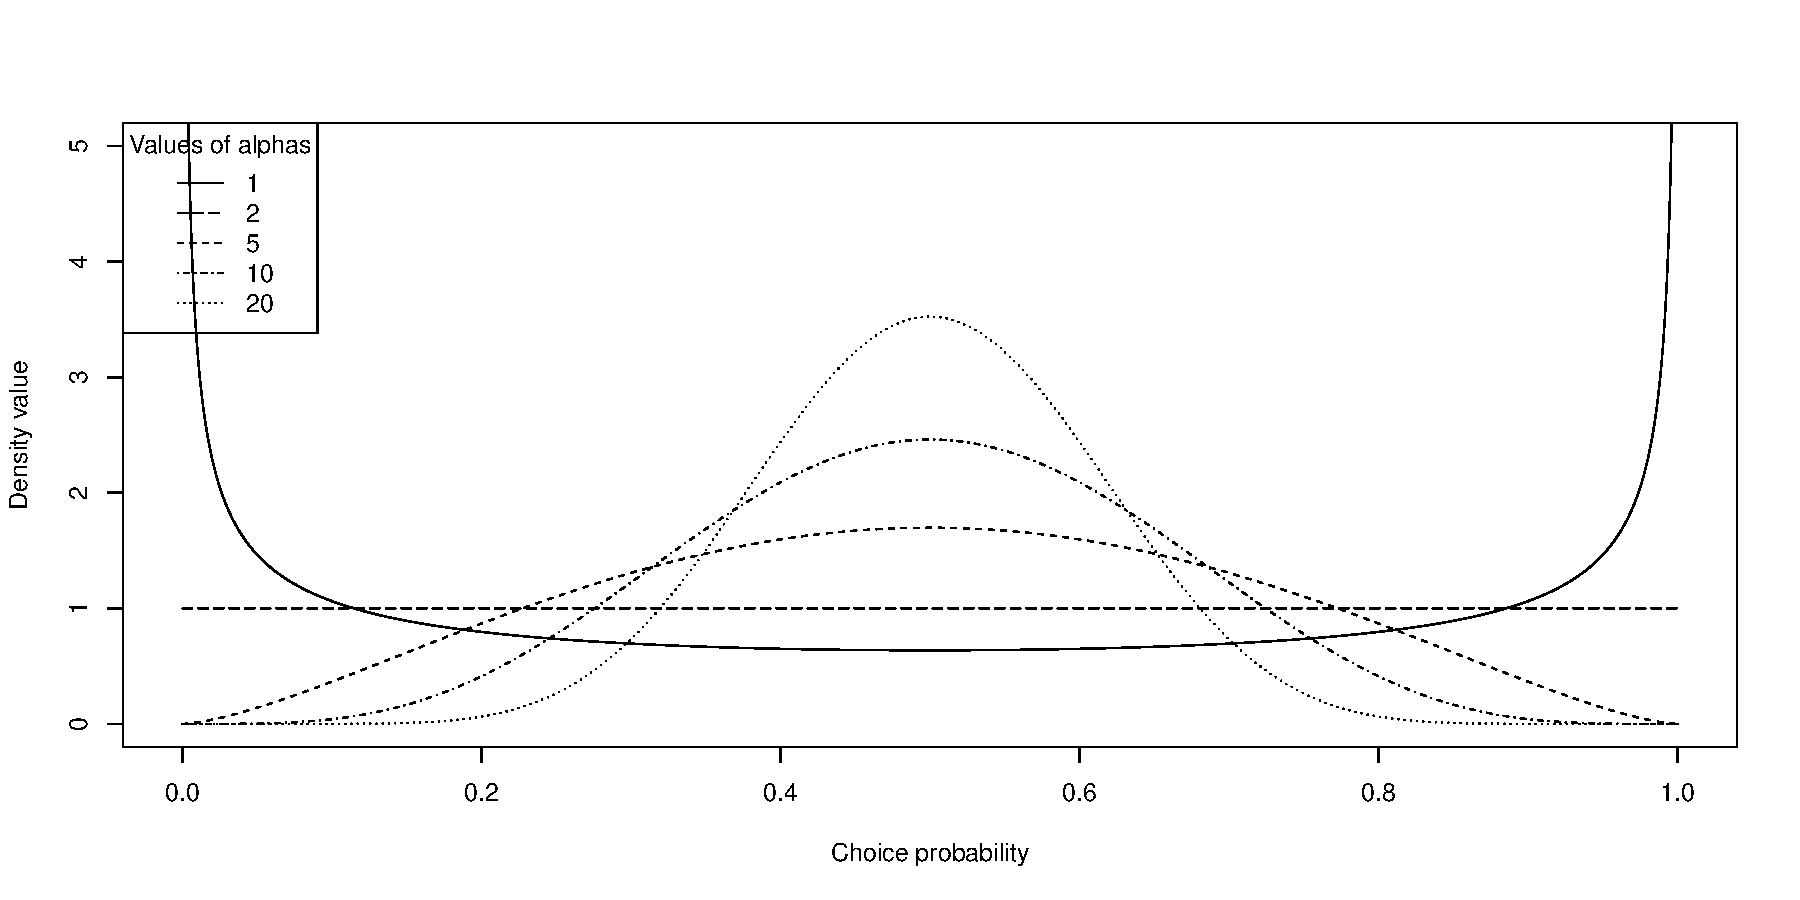
\includegraphics[width=15cm]{Figures/bcp.pdf}
	\caption{Density of binary choice probabilities for $\alpha = 1, 2, 5, 10, 20$}\label{f:bcp}
	\end{center}
\end{figure}

The parameter $\lambda$ describes the degree of dependence of choice probabilities across choice sets.
For $\lambda = 0$, the choice probability vectors $(P_A(x))$ are mutually independent, across $A \subseteq T$.
For $\lambda = 1$, the random choice structure satisfies random utility with probability one.
Mention attractive properties (marginalization condition, anonymity of objects)
Mention empirical support from multi paper.

Don't want to specify $\alpha$, $\lambda$ but rather put a prior on them.
In multi paper, we used several different priors for (alpha, lambda) of the following form, differing in the choices of a0, aA and b: ...
The purpose of this was sensitivity analysis.

We choose different encompassing priors here, partly because of anticipated differences for population choice, partly because of what we learned from previous research.

Population choice is likely to be more central than individual choice.
Choice of prior for alpha: show binary choice probabilities implied by 

We found in the multi paper that lambda is highly relevant.
Our choice of priors in this paper reflects what we found there.
Show different distributions of lambda.







\section{Inferential Methods}\label{s:inference}

For each choice domain, we will describe the posterior distribution of the parameters $\alpha$ and $\lambda$, and compute Bayes factors for comparing the various models described in Section \ref{s:models}.
Both inferential exercises are based on posterior simulation methods outlined in \citeasnoun{McCaMarl14}.

The posterior distribution of the parameters, denoted $\alpha,\lambda|N=n$, represents what we learn, relative to the prior distribution, denoted $\alpha,\lambda$, from a choice experiment.
The posterior distribution is analytically intractable and we use Markov chain Monte Carlo (MCMC) methods to obtain, for a given choice domain, a large posterior sample representing the posterior distribution.
The posterior sample does not consist of independent draws, but there are standard methods for quantifying the simulation error; that is, the difference between posterior sample moments and their population counterparts.
We use the overlapping batch means (OBM) method, whose properties are described in \citeasnoun{FlegJone10}, to compute the numerical standard error of posterior sample means.

We compute Bayes factors for all model comparisons.
Suppose we are comparing two models, $M_1$ and $M_2$, and we observe $N=n$ from a choice experiment.
Then the posterior odds ratio giving the relative posterior probabilities of $M_1$ and $M_2$ can be expressed as
\[
  \frac{\Pr[M_1|N=n]}{\Pr[M_2|N=n]} = \frac{\Pr[M_1]}{\Pr[M_2]}
  \cdot
  \frac{\Pr[N=n|M_1]}{\Pr[N=n|M_2]}
\]
This result follows easily from Bayes' rule and does not depend on how many models are under consideration.
The expression on the right hand side is the product of two factors.
The first is the prior odds ratio and the second is called the {\em Bayes factor}---see \citeasnoun{Berg85} or \citeasnoun{BernSmit94}.
The Bayes factor is a ratio of {\em marginal likelihoods}, and each marginal likelihood $\Pr[N=n|M_i]$ is the probability of observing the data $n$ if the model $M_i$ is true.
Since it makes no reference to any unknown quantities, such as $\alpha$, $\lambda$ or $P$, it can be interpreted as the out-of-sample prediction record of $M_1$ for the data observed.

In the special case where the denominator model is an encompassing model $M_e$ and the numerator model is the constrained model $M_c$ obtained by truncating the density $f(P)$ associated with $M_e$ to the region $\Lambda$ defining an axiom, then the Bayes factor becomes
\begin{equation}\label{e:BF}
  \frac{\Pr[N=n|M_c]}{\Pr[N=n|M_e]} =
  \frac{\Pr[N=n|P \in \Lambda,M_e]}{\Pr[N=n|M_e]} = \frac{\Pr[P \in \Lambda|N=n,M_e]}{\Pr[P \in \Lambda|M_e]}.
\end{equation}

%in principle, this can by computed by marginalizing out the unknown random choice structure $P$:
%\[
%  \Pr[N=n|M_e] = \int_{\Delta} \Pr[N=n|P] f(P) \, dP.
%\]

The second equation of \eqref{e:BF} follows from Bayes' rule; the far right hand side of \eqref{e:BF} is the ratio of posterior to prior probability of the axiom holding in the encompassing model.
A large numerator indicates an axiom that is highly probable in light of the data; a small denominator indicates that an axiom is restrictive.
This ratio also suggests a practical way of computing approximations of Bayes factors: since the probability of an event is just the expectation of an indicator function for the event, we can approximate numerator and denominator using Monte Carlo methods.

\section{Experimental Design}\label{s:design}

The experiment consisted of an internet survey conducted between August 10, 2017 and August 31, 2017.
A total of 1042 respondents completed the survey.

Respondents were recruited by Survey Sampling International (SSI) from their Canadian panel, designed to be representative of the Canadian adult population.
According to the SSI Global Panel Book 2017, included in the experimental supplement to this paper, the Canadian panel consists of 577,356 respondents.
SSI screens respondents for reliability and requires that all respondents be at least 18 years of age.
They also carefully verify the identity of their respondents for each survey.
The Canadian panel is 42\% male and 58\% female and has the following age distribution: the percentage of members in the age range 18-24 is 36\%; 25-34, 25\%; 35-54, 26\%; 55 and older, 13\%.
Compensation of respondents includes cash and other rewards.
The experimental supplement to this paper describes in more detail the recruitment and compensation procedures followed by SSI, although much of the information about these procedures is proprietary.

We imposed no additional restrictions on our sample of respondents.
However, since invited respondents must complete the survey to be included in the sample, there is some self-selection.
We have full information on age, province and sex for all 1042 respondents in our sample.
There are 515 men (49.4\%) and 527 women (50.6\%).
Age ranges from 18 to 88; the percentage of respondents in the age bracket 18-24 is 11.4\%; 25-34, 17.8\%; 35-54, 38.3\%, 55 and older, 32.5\%.
% quartiles of age were 32, 46 and 58.
The number of respondents in Alberta was 124; British Columbia, 136; Manitoba, 36; New Brunswick, 23; Newfoundland and Labrador, 16; Northwest Territories, 1; Nova Scotia, 29; Ontario, 391; Prince Edward Island, 4; Quebec, 251; Saskatchewan, 30; and Yukon, 1.
Respondents could take as long as they liked to complete the survey.
The quartiles of total duration were 7.1, 10.0 and 13.9 minutes.
Three respondents took longer than 24 hours, and the shortest duration was 1.7 minutes

Programming and hosting of the survey were provided by the Institute for Choice at the University of South Australia.

Our experiment features $J=32$ choice domains, including fine art, travel itineraries and pizza toppings.
Each domain consists of a universe of five related choice objects.
The names of the choice domains are shown in Table \ref{t:domains}, together with the question (or an excerpt of the question) used to elicit a response from the participant.
In most cases, this gives an idea of the nature of the choice domain.
Appendix \ref{s:domains} describes each domain in detail, including the question, the five choice objects and, where applicable, a source for the information used to construct the question.
Figure \ref{f:screenshots} shows two different screenshots from the experiment, for the ``Travel'' and ``Coffee'' domains.
There are $I=2^{5}-5-1=26$ choice sets (binary and larger subsets of the five-element universe) for each domain, for a total of $JI=910$ choice sets.
We see in Figure \ref{f:screenshots}, that two of the five choice objects in the ``Travel'' domain and four of the five choice objects in the ``Coffee'' domain are presented to the participant (not at the same time, but rather in two different trials).

\begin{table}[h!]
  \begin{center}
    \caption{Choice domains of the experiment}
    \label{t:domains}
    \begin{small}
    \begin{tabular}{lp{12cm}}
      Domain name & Question\\
      \hline
      	Male stars & Which movie star would you choose to have lunch with? \\
		Female stars & Which movie star would you choose to have lunch with? \\
		Films & Judging from the following descriptions of films, which one of the films would you choose to see? \\
		Star pairs & Knowing only who is starring, which one of these new films would you choose to see? \\
		Pizzas & Which one of the following pizzas would you choose? \\
		Juices & Which one of the following fresh juices would you choose? \\
		Colours & Which one of the following colours do you like best? \\
		Colour Pairs & Which one of these colour combinations do you like best? \\
		Events & Which one of the following events do you think is most likely to happen in the next twenty years? \\
		Radio formats & Suppose you were on a two hour road trip and you have a choice among radio stations with the following formats.
Which one would you choose? \\
		Music & Which one of the following musical artists do you like the best? \\
		Aborig. art & Which one of the following examples of Australian aboriginal art do you like the best? \\
		Impress. art & Which one of the following examples of Impressionist art do you like the best? \\
		Sentences & Which one of the following sentences do you find the most grammatically acceptable? \\
		Travel & Which one of the following travel destinations would you most like to visit? \\
		Marijuana & Which one of the following marijuana policies would you choose? \\
		Latitude & Which one of the following cities do you think is furthest north? \\
		Dots & Which one of the following boxes do you think has the greatest number of points? \\
		Triangles & Which one of the following triangles do you think has the greatest area? \\
		Population & Which one of the following countries do you think has the largest population? \\
		Area & Which one of the following countries do you think has the greatest surface area, including inland bodies of water? \\
		Beer & ... Given that you had to choose one brand to buy on this information alone, which one would you choose? \\
		Cars & Which one of the following cars would you choose to drive, all other features
begin equal? ... \\
		Restaurants & Which one of the following restaurants would you choose for your next restaurant meal...? \\
		Itineraries I & Which one of the following flight itineraries would you choose? ... \\
		Payoffs & Which one of the following would you choose? \\
		Phone plans & Of the following cell phone plans, which one would you choose? ... \\
		Hotel rooms & ... Which one of the following hotels would you choose, ...? \\
		Itineraries II & Which one of the following flight itineraries would you choose? ... \\
		Televisions & Which one of the following televisions would you choose to buy ...? \\
		Coffee & Which one of the following ground coffees would you choose? \\
		Charity & Suppose someone was donating a total of 100 dollars to a combination of charities,
on your behalf.
Which one of the following divisions of the 100 dollars would you choose? \\
    \end{tabular}
    \end{small}
  \end{center}
\end{table}

Our design is strictly between-subject.
Within each domain, each of the $I$ choice sets is presented exactly $N=40$ times, once to each of $N$ distinct respondents.
Each respondent faces exactly one choice set from each domain, for a total of $J$ trials.
Thus the total number of respondents is $NI=1040$, and the total number of trials is $NIJ=33,280$.
Respondents must choose exactly one object from each choice set.
In some trials, respondents select radio buttons and in other trials, respondents select pictures, which are then identified by a border.
In each case, respondents can modify their choice before they confirm it by clicking on a button labelled ``$>>$''; once they click this button, they cannot go back and change their response.
Figure \ref{f:screenshots} shows a screenshot of a domain with pictures and one of a domain with radio buttons.

\begin{figure}
	\begin{center}
	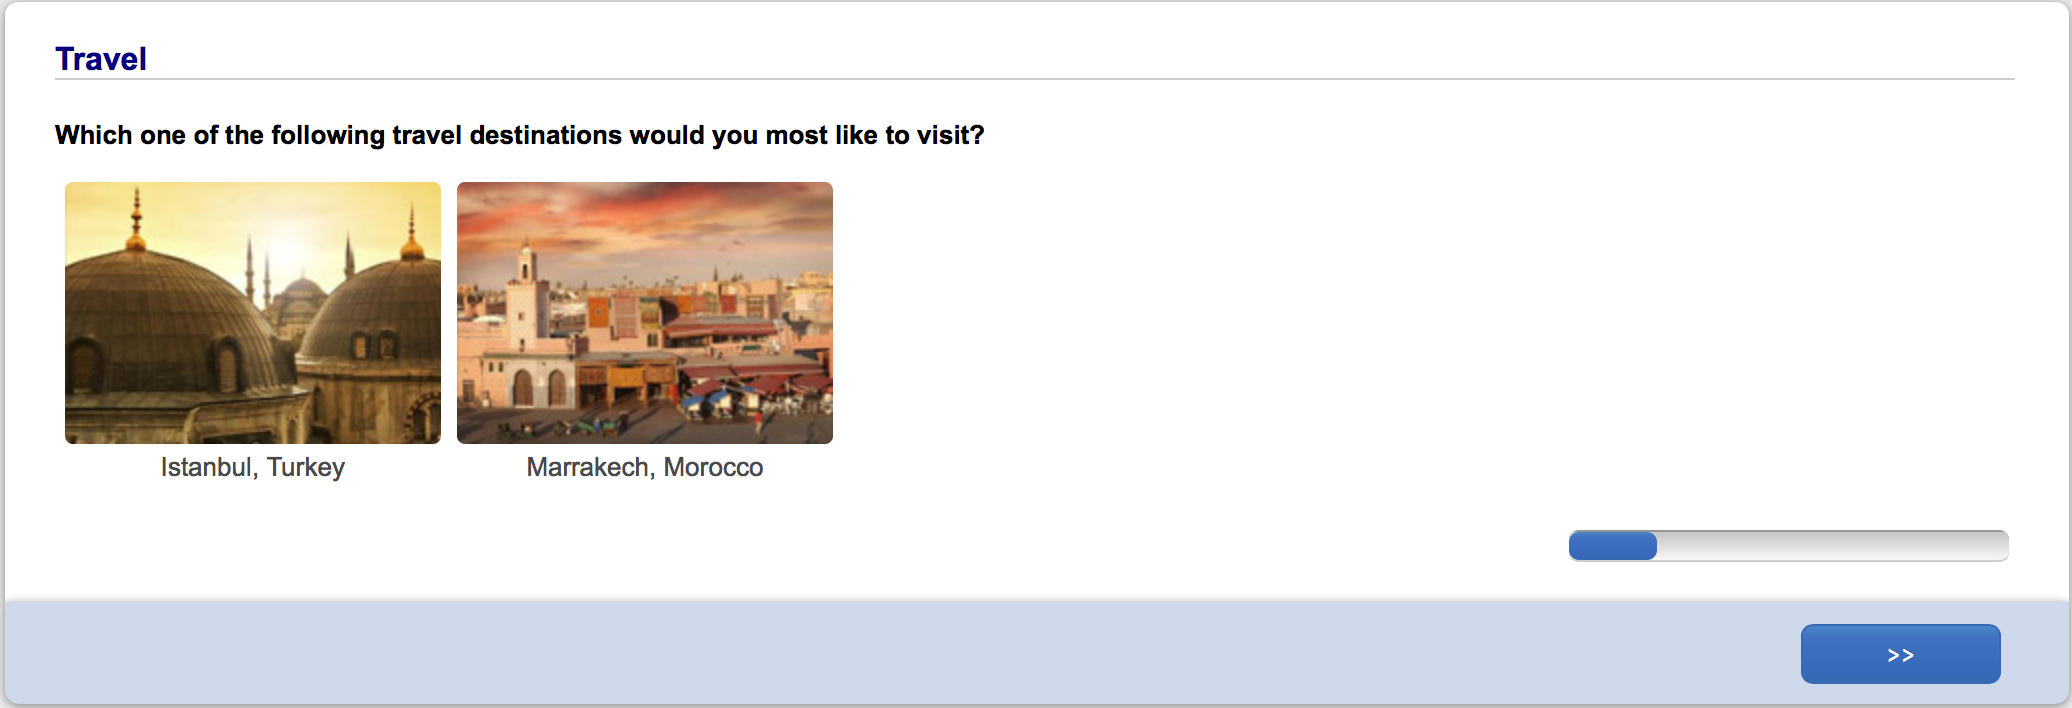
\includegraphics[width=15cm]{Population_study_design/screenshot_Travel.png}
	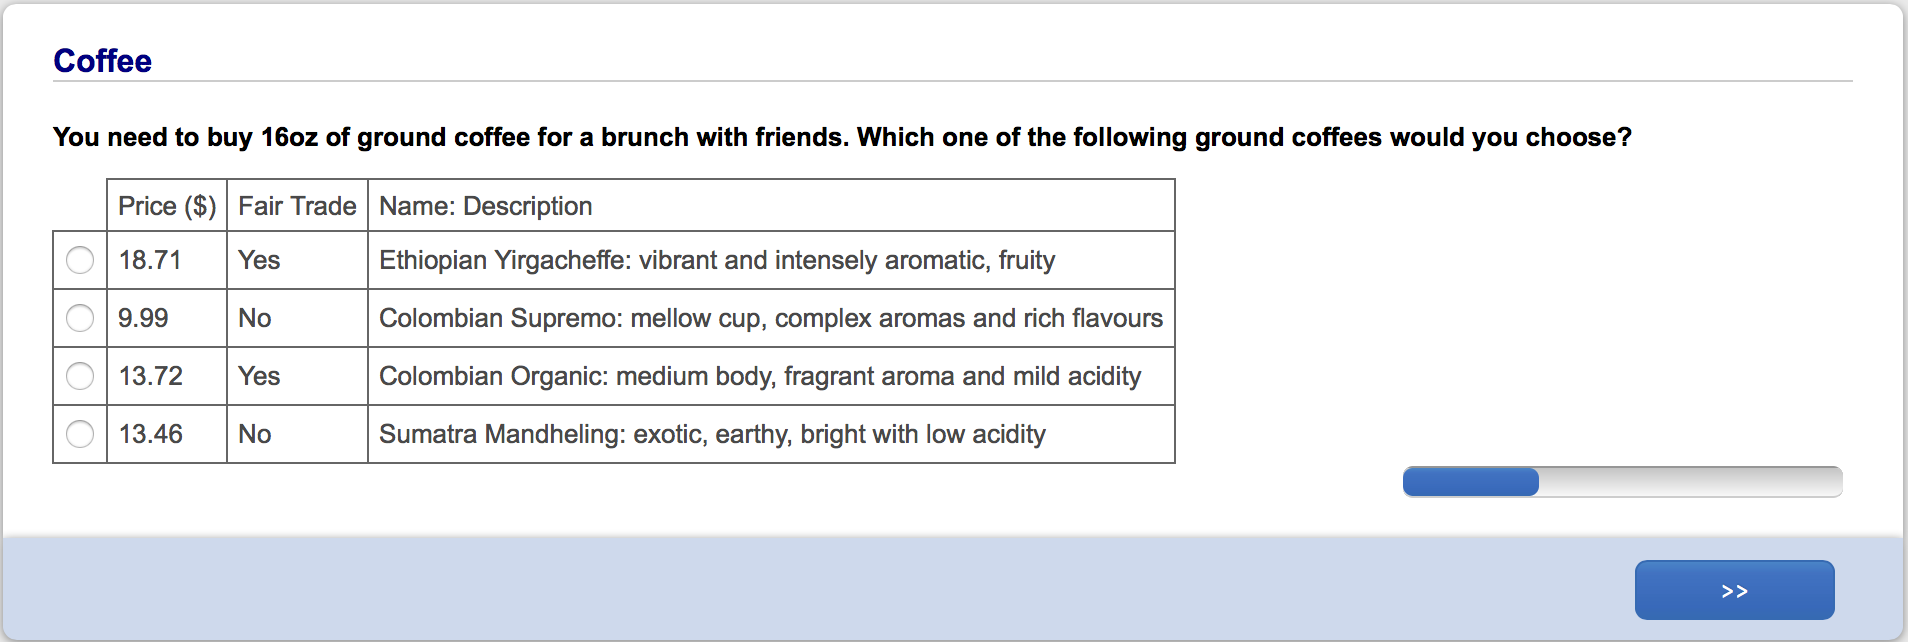
\includegraphics[width=15cm]{Population_study_design/screenshot_Coffee.png}
	\caption{A screenshot for the ``Travel'' domain, in which respondents select pictures, and a screenshot for the ``Coffee'' domain, in which respondents select radio buttons. In the experiment, these photographs are in colour.}\label{f:screenshots}
	\end{center}
\end{figure}

For each domain $j$, the $NI$ respondents are randomly partitioned into $I$ groups of size $N$, with respondents in each group seeing the same choice set from that domain.
Random partitions are uniformly distributed and mutually independent across domains.
Elements of a choice set are presented in random position (left, middle, right, for example) on the screen, independently across the $N$ respondents facing that choice set.
The $J$ trials assigned to each respondent are presented in random
order, with order independent across respondents.
Random partitions, positions and trial order are mutually independent.

\section{Results}\label{s:results}

\begin{figure}
	\begin{center}
	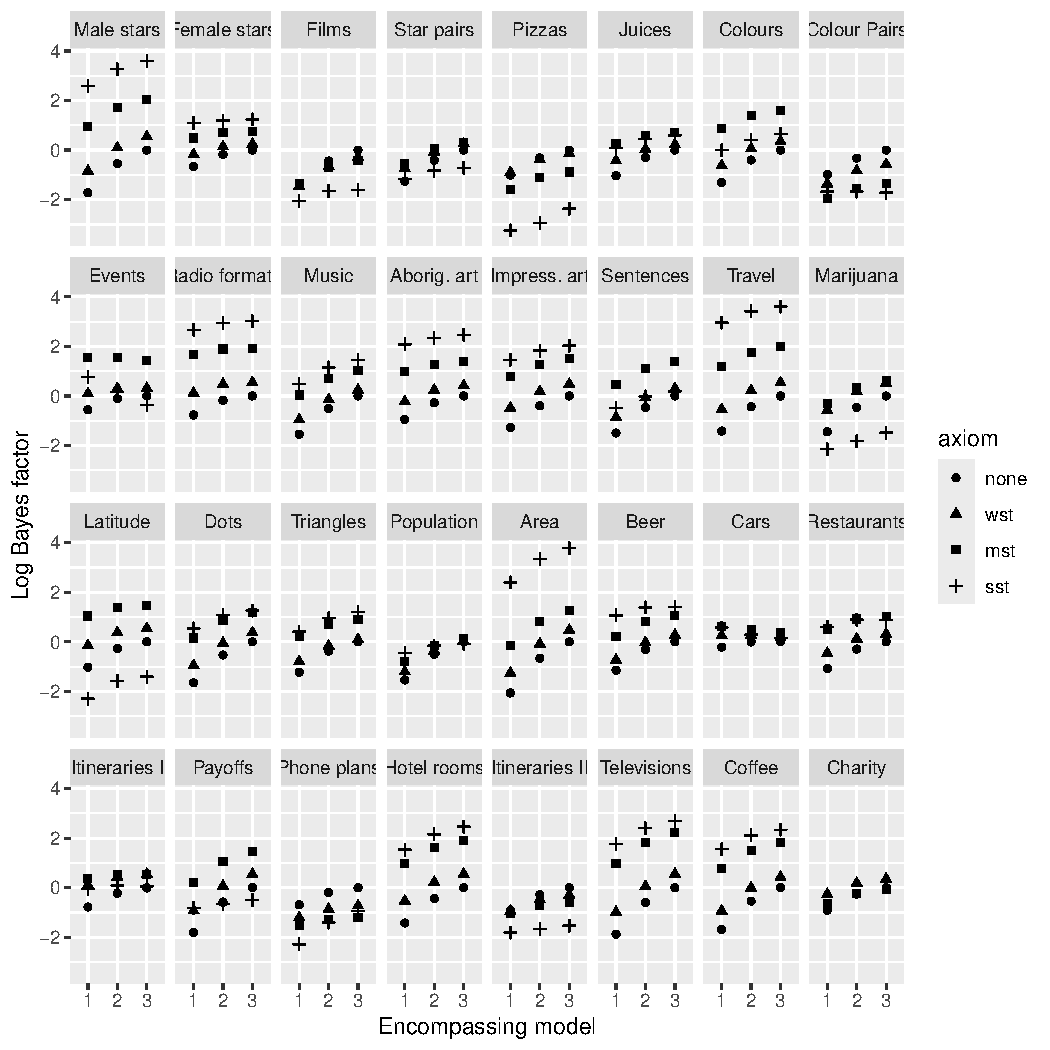
\includegraphics[width=16cm]{Figures/binary_BF}
	\caption{Log Bayes factors for 32 domains, by encompassing model and binary choice axiom}\label{f:binary_BF}
	\end{center}
\end{figure}

\begin{figure}
	\begin{center}
	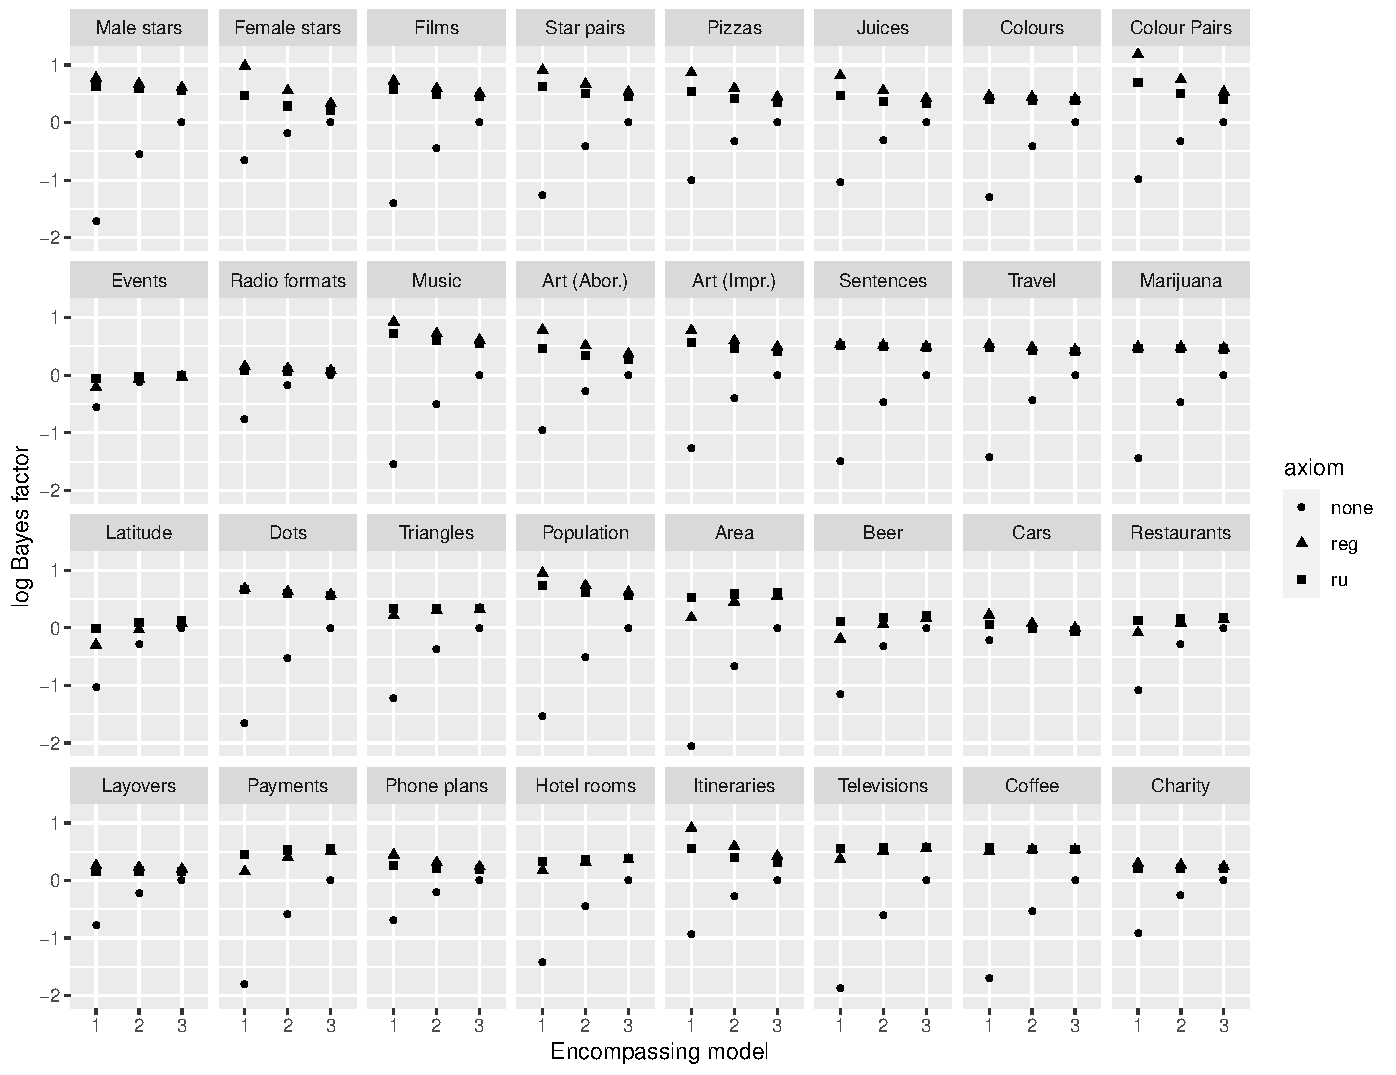
\includegraphics[width=16cm]{Figures/multiple_BF}
	\caption{Log Bayes factors for 32 domains, by encompassing model and multiple choice axiom}\label{f:multiple_BF}
	\end{center}
\end{figure}


\subsection{Graphical Illustrations}

Figure \ref{f:colours} illustrates binary and ternary choice probabilities, as they relate to regularity and the multiplicative inequality, for the ``Colours'' domain.
The figure consists of 10 panels, with each panel corresponding to one of the ten tripleton choice sets from that domain.

Each panel features an equilateral triangle, with vertices labelled with three of the choice objects from the domain.
Take the first panel as an example, where the vertices are labelled $a$ (bottom left) $b$ (top) and $c$ (bottom right).
Each point in the triangle, including the interior and the boundary, represents a triple $(P_A(a),P_A(b),P_A(c))$ of choice probabilities, in a Barycentric coordinate system.
Thus, the distance of a point to the right side of the triangle gives $P_A(a)$, the distance to the base gives $P_A(b)$ and the distance to the left side gives $P_A(c)$.
The point is also the convex combination of the vertices $a$, $b$ and $c$---which have Barycentric coordinates $(1,0,0)$, $(0,1,0)$ and $(0,0,1)$, respectively---with weights $P_A(a)$, $P_A(b)$ and $P_A(c)$.

The hollow dots on the left, right and bottom sides of the triangle represent the binary probabilities $p(a,b)$, $p(b,c)$ and $p(a,c)$, respectively.
For example, the dot on the left side of the triangle is the convex combination of the vertices labelled $a$ and $b$, with weights $p(a,b)$ and $p(b,a)$ respectively.
Throughout, we reserve hollow dots for binary probabilities and solid dots for ternary probabilities, to avoid any ambiguity for points on the boundary of the triangle.

The blue triangle in each figure gives necessary conditions on the ternary probability, given the three binary probabilities, for regularity to hold: ternary probabilities within the blue triangle satisfy $P_A(a) \leq \min(p(a,b), p(a,c)$, $P_A(b) \leq \min(p(b,a), p(b,c))$ and $P_A(c) \leq \min(p(c,a), p(c,b))$.
Similarly, the red triangle gives necessary conditions on the ternary probability, give the binary probabilities, for the multiplicative inequality to hold: here the conditions are $P_A(a) \geq p(a,b) p(a,c)$, $P_A(b) \geq p(b,a), p(b,c)$ and $P_A(c) \geq p(c,a), p(c,b)$.

\begin{figure}
	\caption{Binary and ternary probabilities for the Colours domain.}\label{f:colours}
	\centering
	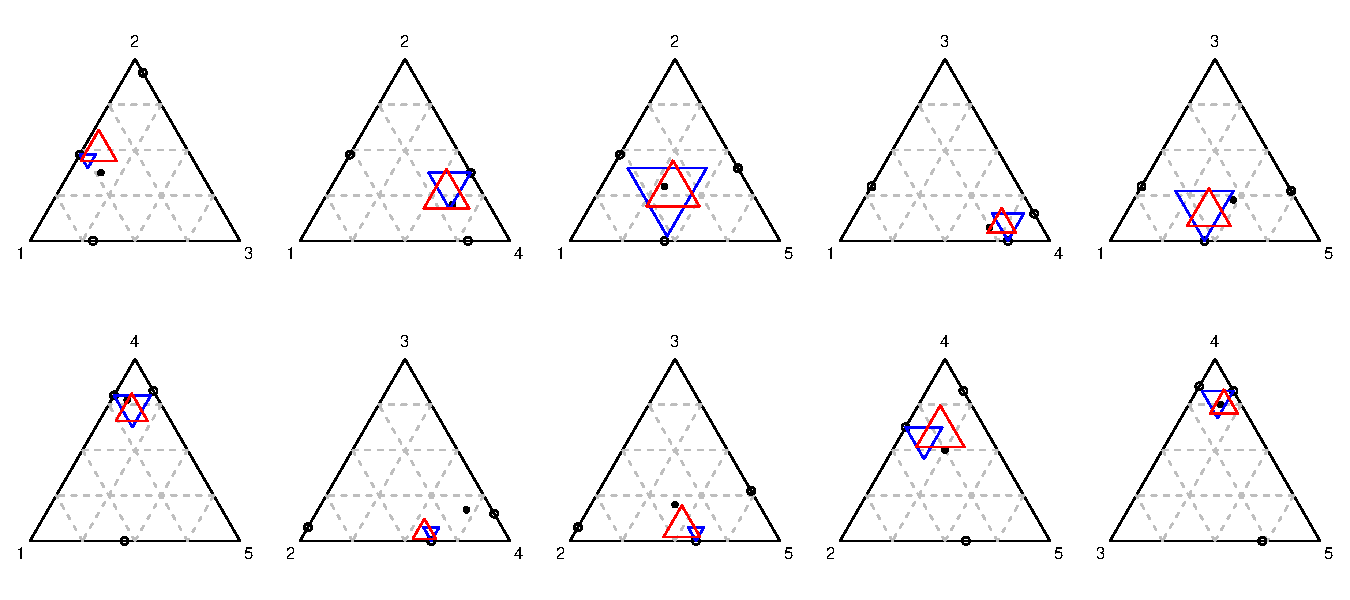
\includegraphics[width=16cm]{./Population_study_data/Simplexes/Colours.pdf}
\end{figure}

\subsection{Evaluating axioms using formal model comparison tools}

In this section we tests axiom by measuring how much the predictive performance of an unrestricted model of choice probabilities improves when we impose the restriction implied by the axiom.
Given some observed choice data $y$, the Bayes factor in favour of the restricted model, relative to the unrestricted model, is the ratio of the probability of $y$ occurring under the restricted model to the probability of $y$ occurring under the unrestricted model.
Letting $\Lambda$ be the event that the axiom holds, we can express this Bayes factor as the ratio on the left hand side of equation \eqref{e:BFidentity}.
\begin{equation}\label{e:BFidentity}
	\frac{\Pr[y|\Lambda]}{\Pr[y]} = \frac{\Pr[\Lambda|y]}{\Pr[y]}.
\end{equation}

Now by Bayes rule, we obtain the equality in \eqref{e:BFidentity}.
The ratio on the right hand side is something we can estimate by simulation.
It is the ratio of posterior to prior probability that the axiom holds, under the unrestricted model.
High posterior probability in the numerator favours an axiom that is compatible with observed choice frequencies; low prior probability in the denominator favours an axiom that is restrictive, a kind of model parsimony.

In order to obtain prior and posterior probabilities of an axiom, we must decide on a prior distribution for $P$.
We use a set of nine hierarchical prior distributions described in \citeasnoun{McCaMarl13} in order to assess the robustness of our results to the prior specification.
Each of these priors is symmetric with respect to choice objects and has full support on the space of random choice structures.

We compute prior and posterior probabilities of axioms numerically using the similation methods described in \citeasnoun{McCaMarl14}.
We compute numerical standard errors of prior and posterior probabilities using the overlapping batch mean method described in \citeasnoun{FlegJone10} and combine these standard errors to compute standard errors for Bayes factors using the delta method.

\section{Conclusions}\label{s:conclude}

\appendix

\section{Definitions of axioms and basic results}\label{s:axioms}

A random choice structure satisfies
\begin{description}
	\item[WST] {\em weak stochastic transitivity} if and only if for all distinct
	$x$, $y$ and $z$,
	\[
		p(x,y) \geq \frac{1}{2}\;\mbox{and}\; p(y,z) \geq \frac{1}{2}
		\Rightarrow p(x,z) \geq \frac{1}{2},
	\]
	\item[MST] {\em moderate stochastic transitivity} if and only if for all distinct
	$x$, $y$ and $z$,
	\[
		p(x,y) \geq \frac{1}{2}\;\mbox{and}\; p(y,z) \geq \frac{1}{2}
		\Rightarrow p(x,z) \geq \min[ p(x,y), p(y,z) ],
	\]
	\item[SST] {\em strong stochastic transitivity} if and only if for all distinct
	$x$, $y$ and $z$,
	\[
		p(x,y) \geq \frac{1}{2}\;\mbox{and}\; p(y,z) \geq \frac{1}{2}
		\Rightarrow p(x,z) \geq \max[ p(x,y), p(y,z) ],
	\]
	\item[TI] the {\em triangle inequality} if and only if for all distinct
	$x$, $y$ and $z$,
	\[
		p(x,y) + p(y,z) + p(z,x) \geq 1,
	\]
	\item[Reg] {\em regularity} if and only if for all $x \in A \subseteq B \subseteq T$,
	\[
		P_A(x) \geq P_B(x),
	\]
	\item[MI] the {\em multiplicative inequality} if and only if for all $x \in A, B \subseteq T$,
	\[
		P_{A \cup B} \geq P_A(x) P_B(x),
	\]
	\item[FI] the {\em Falmagne inequalities} if and only if for all non-empty
	$A \subseteq T$ and all $x \in A$,
	\begin{equation}\label{e:BMP}
		\sum_{B \colon A \subseteq B \subseteq T} (-1)^{|B \backslash A|} P_B(x) \geq 0.
	\end{equation}
\end{description}

The multiplicative inequality is due to \citeasnoun{SattTver76}, who show that it is a testable implication of the Elimination by Aspects model described in \citeasnoun{Tver72a} and \citeasnoun{Tver72b} and the independent random utility model.

%%%%%%%%%%%%%%%%%%%%%%%%%%%%%%%%%%%%%%%%%%%%%%%%%
%%%%%%%%%%%%%%%%%%%%%%%%%%%%%%%%%%%%%%%%%%%%%%%%%
%%%%%%%%%%%%%%%%%%%%%%%%%%%%%%%%%%%%%%%%%%%%%%%%%
% DOMAINS
%%%%%%%%%%%%%%%%%%%%%%%%%%%%%%%%%%%%%%%%%%%%%%%%%
%%%%%%%%%%%%%%%%%%%%%%%%%%%%%%%%%%%%%%%%%%%%%%%%%
%%%%%%%%%%%%%%%%%%%%%%%%%%%%%%%%%%%%%%%%%%%%%%%%%

\section{Domains}\label{s:domains}

Here, we describe a set of $J$ choice domains.

We classify choice domains into four categories.
In the first category, objects have no numerical attributes.
In the second category, objects have a single attribute, whose level is not explicitly given. In the third category, objects have two numerical attributes and the experimental design is intended to elicit one or more context effects.
In the fourth category, objects have many attributes, and they are chosen to resemble objects in discrete choice experiments used in Marketing, although with fewer attributes.

The section titles, ``Male stars'' for example, give the names of the domains for the purpose of reporting results.
The specification of a domain is shown in a grey box and consists of a question and five choice objects, or responses.
In the actual experiment, for a given domain, all respondents see the same question (such as ``Which movie star would you choose to have lunch with?'') but not the same set of responses; different respondents will see from two to five of the possible responses, in random order, as described in Section \ref{s:design}.
For the purpose of reporting results, the choice objects in each domain are labelled $a$, $b$, $c$, $d$ and $e$, in the order presented in the grey boxes.
The respondents do not see these labels, and accordingly, we do not use them within the boxes.

We adopt the convention that whenever there is an established order for the items in a list, we order them in decreasing order.
Again, this is only for the purposes of reporting results; each respondent sees the items in a choice set in random order.

\subsection{No numerical attributes}

\subsubsection{Male stars}

% Male stars

The source for this domain is the website \texttt{ranker.com}, accessed June 4, 2017.
The list is ``The best actors working today''.
The choices are the top five actors in that list, in order.

\begin{tcolorbox}
Which movie star would you choose to have lunch with?

\begin{itemize}
	\setlength\itemsep{-5pt}
	\item Tom Hanks
	\item Kevin Spacey
	\item Morgan Freeman
	\item Leonardo DiCaprio
	\item Christian Bale
\end{itemize}
\end{tcolorbox}

\subsubsection{Female stars}

% Female stars

The source for this domain is the website \texttt{ranker.com}, accessed June 4, 2017.
The list is ``The best American actresses working today''.
These are the top five actors in that list, in order.
Jodie Foster's name was misspelled in the experiment, as two participants noted in the comments.

\begin{tcolorbox}
Which movie star would you choose to have lunch with?

\begin{itemize}
	\setlength\itemsep{-5pt}
	\item Meryl Streep
	\item Jody Foster
	\item Kathy Bates
	\item Amy Adams
	\item Julianne Moore
\end{itemize}
\end{tcolorbox}


\subsubsection{Films}

% Films

The source for this domain is the IMDb list ``Most Popular Feature Films Released 1990 to
1999''.
The decade was chosen so that the films would not be easily recognizable by most respondents.

\begin{tcolorbox}
Judging from the following descriptions of films, which one of the films would you choose to see?

\begin{itemize}
	\setlength\itemsep{-15pt}
	\item Two imprisoned men bond over a number of years, finding solace and
eventual redemption through acts of common decency. \\
	\item Mathilda, a 12-year-old girl, is reluctantly taken in by L\'eon, a
professional assassin, after her family is murdered. L\'eon and Mathilda
form an unusual relationship, as she becomes his prot\'eg\'e and learns the
assassin's trade. \\
	\item The lives of two mob hit men, a boxer, a gangster's wife, and a pair
of diner bandits intertwine in four tales of violence and redemption. \\
	\item A sexually frustrated suburban father has a mid-life crisis after
becoming infatuated with his daughter's best friend. \\
	\item Identical twins, separated at birth and each raised by one of their
biological parents, discover each other for the first time at summer camp
and make a plan to bring their wayward parents back together.
\end{itemize}
\end{tcolorbox}


\subsubsection{Star pairs}

% Star pairs

Here, choice objects are pairs of movie stars from a set of four movie stars: Tom Hanks, Scarlett Johansson, Brad Pitt and Angelina Jolie.
The only missing pair is Brad Pitt and Angelina Jolie.
One possible measure of similarity is the number of actors in common between two pairs, with values 0 and 1.
There are nine doubleton choice sets (i.e. pairs of actor pairs) with one star in common and one ($\{c,d\}$) without any stars in common.
Thus there are three triples ($\{a,c,d\}$, $\{b,c,d\}$, $\{c,d,e\}$) where one might expect a similarity effect.

In this example, respondents' preferences may depend not only on their liking of particular actors but also on complementaries between actors.
{}
\begin{tcolorbox}
Knowing only who is starring, which one of these new films would you choose to see?

\begin{itemize}
	\setlength\itemsep{-5pt}
	\item Tom Hanks and Scarlett Johansson
	\item Scarlett Johansson and Brad Pitt
	\item Tom Hanks and Brad Pitt
	\item Scarlett Johansson and Angelina Jolie
	\item Tom Hanks and Angelina Jolie
\end{itemize}
\end{tcolorbox}


\subsubsection{Pizzas}

% Pizzas

The source for this domain is a Montreal pizza restaurant.
All these pizzas are either 12 or 13 dollars.

\begin{tcolorbox}
Which one of the following pizzas would you choose?

\begin{itemize}
	\setlength\itemsep{-5pt}
	\item Mozzarella, tomato sauce, basil
	\item Pepperoni, mushrooms, green pepper, mozzarella, tomato sauce
	\item Red onion, tomato sauce, feta, mozzarella, olive oil, Greek spices,
tomato sauce
	\item Bacon, white onion, mozzarella, parmesan, fresh cream, tomato sauce,
ground pepper
	\item Mushrooms, green pepper, mozzarella, tomato sauce
\end{itemize}
\end{tcolorbox}


\subsubsection{Juices}

% Juices

\begin{tcolorbox}
Which one of the following fresh juices would you choose?

\begin{itemize}
	\setlength\itemsep{-5pt}
	\item Mango
	\item Orange
	\item Apple
	\item Grapefruit
	\item Pineapple
\end{itemize}
\end{tcolorbox}


\subsubsection{Colours}

% Colours

\begin{tcolorbox}
Which one of the following colours do you like best?

\begin{itemize}
	\setlength\itemsep{-5pt}
	\item Red
	\item Purple
	\item Pink
	\item Blue
	\item Green
\end{itemize}
\end{tcolorbox}


\subsubsection{Colour pairs}

% Colour pairs

The source for this domain is the website ``The top tens'', page ``Two colors that look good side by side.''
The color combinations here are ranked 1, 4, 5, 13 and 14.
We chose a selection of five high ranking combinations among which there were many colors
in common.
Using a similarity measure equal to the number of colours in common between two pairs, there are two doubleton choice sets where the two colour pairs have no colours in common ($\{a,e\}$ and $\{b,d\}$) and eight where the two colour pairs have one colour in common.
This gives six tripleton pairs in which one might expect a similarity effect.

\begin{tcolorbox}
Which one of these colour combinations do you like best?

\begin{itemize}
	\setlength\itemsep{-5pt}
	\item Black and red
	\item Black and purple
	\item Black and blue
	\item Blue and red
	\item Blue and purple
\end{itemize}
\end{tcolorbox}


\subsubsection{Events}

% Events

This domain involves comparisons of the probabilities of future events.
Logically, the probability of event e must be as least as great as the probability of a, which must in turn be as least as great as the probability of d; also, the probability of b must be at least as great as the probability of c.
There is potential for several asymmetric dominance effects in this domain, based on these dominance relations.
These would be unconventional effets, as most experimental designs in the literature intended to elicit asymmetric dominance effects feature numerical dominance relations.

\begin{tcolorbox}
Which one of the following events do you think is most likely to happen in the next twenty years?

\begin{itemize}
	\setlength\itemsep{-5pt}
	\item Scotland becomes an independent country.
	\item Either Catalonia or Quebec become independent countries.
	\item Catalonia becomes an independent country.
	\item Scotland and Quebec become independent countries.
	\item Either Scotland or Quebec become independent countries.
\end{itemize}
\end{tcolorbox}


\subsubsection{Radio formats}

% Radio formats

The domain is radio formats, and the choice objects are the top 5 radio formats in Canada in 2015, according to
\begin{quotation}
	https://byrnesmedia.com/2015/10/05/the-6-best-performing-radio-formats-in-canada/
\end{quotation}
Descriptions of formats are from
\begin{quotation}
	http://www.newsgeneration.com/broadcast-resources/guide-to-radio-station-formats/
\end{quotation}

\begin{tcolorbox}
Suppose you were on a two hour road trip and you have a choice among radio stations with the following formats.
Which one would you choose?

\begin{itemize}
	\setlength\itemsep{-5pt}
	\item News
	\item Hot Adult Contemporary, or Hot AC
	(A variety of classic and contemporary mainstream music geared towards adults.)
	\item Classic Hits (Rock and pop, roughly 1964-1989)
	\item Country Music
	\item Adult Contemporary, or AC (Adult-oriented pop/rock with no hard rock.)
\end{itemize}
\end{tcolorbox}


\subsubsection{Musical artists}

% Musical artists

The choice objects in this domain are the top selling musical artists of all time, according to Wikipedia.
They should be familiar to a large majority of respondents.

\begin{tcolorbox}
Which one of the following musical artists do you like the best?

\begin{itemize}
	\setlength\itemsep{-5pt}
	\item The Beatles
	\item Elvis Presley
	\item Michael Jackson
	\item Madonna
	\item Elton John
\end{itemize}
\end{tcolorbox}


\subsubsection{Aboriginal art}

% Aboriginal art

\begin{tcolorbox}
Which one of the following examples of Australian aboriginal art do you like the best?


\includegraphics[width=3cm]{Population_study_design/Aboriginal_art1.jpg}
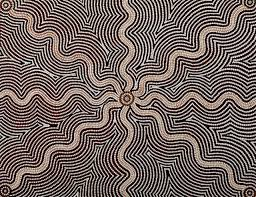
\includegraphics[width=3cm]{Population_study_design/Aboriginal_art2.jpg}

\includegraphics[width=3cm]{Population_study_design/Aboriginal_art3.jpg}

\includegraphics[width=3cm]{Population_study_design/Aboriginal_art4.jpg}

\includegraphics[width=3cm]{Population_study_design/Aboriginal_art5.jpg}
\end{tcolorbox}


\subsubsection{Impressionist art}

% Impressionist Art

\begin{tcolorbox}
Which one of the following examples of Impressionist art do you like the best?

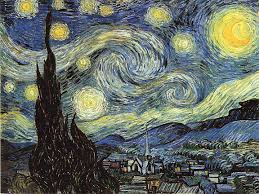
\includegraphics[width=3cm]{Population_study_design/Impressionist_art1.jpg}

\includegraphics[width=3cm]{Population_study_design/Impressionist_art2.jpg}
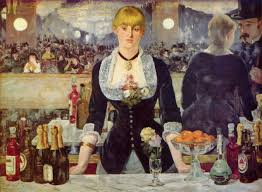
\includegraphics[width=3cm]{Population_study_design/Impressionist_art3.jpg}
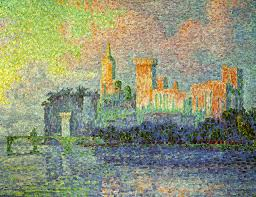
\includegraphics[width=3cm]{Population_study_design/Impressionist_art4.jpg}

\includegraphics[width=3cm]{Population_study_design/Impressionist_art5.jpg}
\end{tcolorbox}


\subsubsection{Sentences}

% Sentences

This domain consists of sentences that have been used in experiments of linguistic judgement.
They are, respectively sentences 7j, 7h, 7p, 7a and 7e in \citeasnoun{BardRobeSora96}.
Figure 1 of that paper shows acceptability scores for these and other sentences given by two individual linguists, an acceptability score aggregating the scores of four linguists and an acceptability score aggregating the scores of four ``naive respondents'', all undergraduate anatomy students.
There is broad, but not perfect, agreement in terms of order, and in the following list, they are in decreasing order of acceptability according to the measure aggregating the judgements of four linguists.

\begin{tcolorbox}
Which one of the following sentences do you find the most grammatically acceptable?

\begin{itemize}
	\setlength\itemsep{-5pt}
	\item Who did Bill buy the car to please?
	\item This is a book which reading would be fun.
	\item Where did Bill buy the car to drive?
	\item Which man do you wonder when to meet?
	\item With which pen do you wonder what to write?
\end{itemize}
\end{tcolorbox}


\subsubsection{Travel}

% Travel

The source is Tripadvisor.
These are the top five travel destinations, according to the results of an on-line contest where visitors to a Tripadvisor site could make pairwise choices between travel destinations.

\begin{tcolorbox}
\begin{quotation}
Which one of the following travel destinations would you most like to visit?
\end{quotation}

\begin{enumerate}
\item Marrakech, Morocco

\includegraphics[height=2.8cm]{Population_study_design/Travel1.jpg}

\item Istanbul, Turkey

\includegraphics[height=2.8cm]{Population_study_design/Travel2.jpg}

\item Hanoi, Vietnam

\includegraphics[height=2.8cm]{Population_study_design/Travel3.jpg}

\item Siem Reap, Cambodia

\includegraphics[height=2.8cm]{Population_study_design/Travel4.jpg}

\item Praque, Czech Republic

\includegraphics[height=2.8cm]{Population_study_design/Travel5.jpg}
\end{enumerate}	
\end{tcolorbox}


\subsubsection{Marijuana}

% Marijuana

This question elicits policy preferences.

\begin{tcolorbox}
Which one of the following marijuana policies would you choose?

\begin{itemize}
	\setlength\itemsep{-5pt}
	\item Possession by, and sales to adults are both legal; sales to minors are illegal.
	\item Possession by, and sales to adults are both illegal but neither is a criminal offense; sales to minors are a criminal offense.
	\item Possession is illegal but not criminal; all sales are a criminal offense.
	\item Possession and sales are criminal offenses, with a small number of medical exceptions.
	\item Possession and sales are criminal offenses, without exception.
\end{itemize}
\end{tcolorbox}


\subsection{Single attributes, not directly observed}

The five domains in this section contain choice objects with an objective rank order.

\subsubsection{Latitude}

% Latitude

The five cities of this domain have a latitude close to 50 degrees north.
In the following list, they are ordered from furthest north to furthest south.
According to Wikipedia, their latitudes are, respectively, $52\degree14^\prime N$, $51\degree30^\prime N$, $49\degree15^\prime N$, $48\degree51^\prime N$ and $47\degree36^\prime N$.
There are two potential asymmetric dominance effects, with Vancouver being fairly obviously north of Seattle and London being fairly obviously north of Paris.

\begin{tcolorbox}
Which one of the following cities do you think is furthest north?

\begin{itemize}
	\setlength\itemsep{-5pt}
	\item Warsaw, Poland
	\item London, United Kingdom
	\item Vancouver, Canada
	\item Paris, France
	\item Seattle, United States
\end{itemize}
\end{tcolorbox}


\subsubsection{Dots}

% Dots

This domain is a perception example.
The true numbers of points are, respectively, 320, 310, 300, 290 and 280.
It is much clearer that there are more points in the first panel than in the fifth, than that there are more points in the first than in the second.
The difference in the number of points is an obvious similarity measure here that might be expected to lead to similarity effects.
{}
\begin{tcolorbox}
Which one of the following boxes do you think has the greatest number of points?

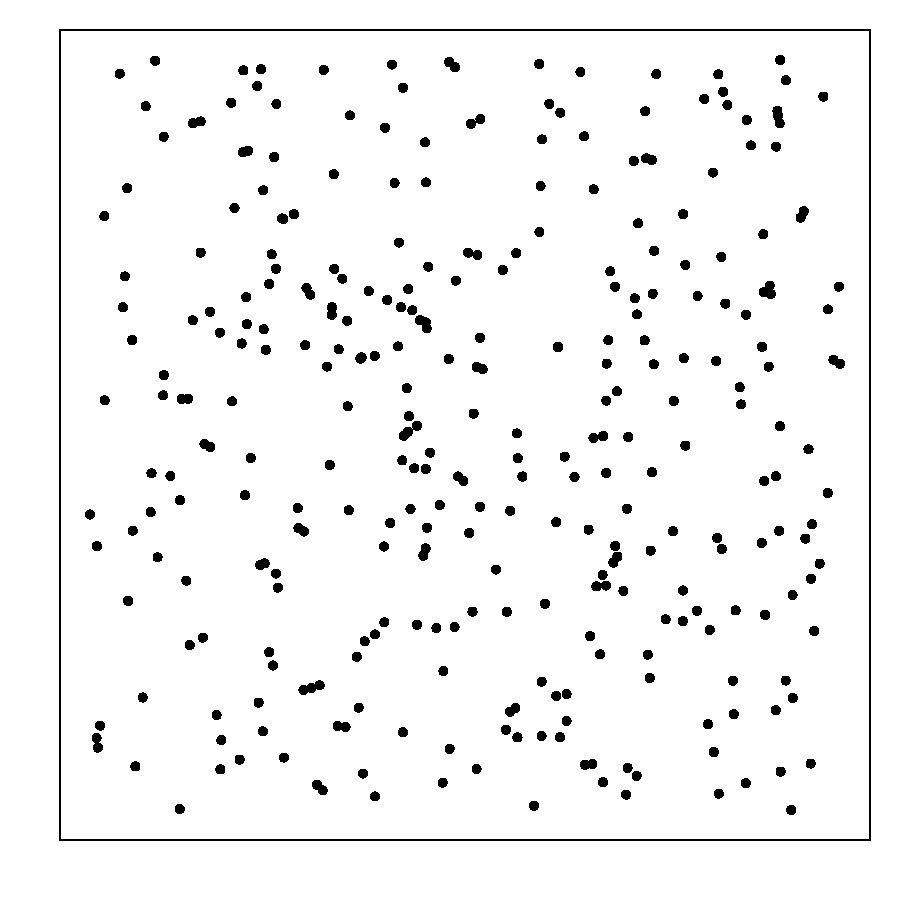
\includegraphics[height=3cm]{Population_study_design/Scatterplots1.pdf}
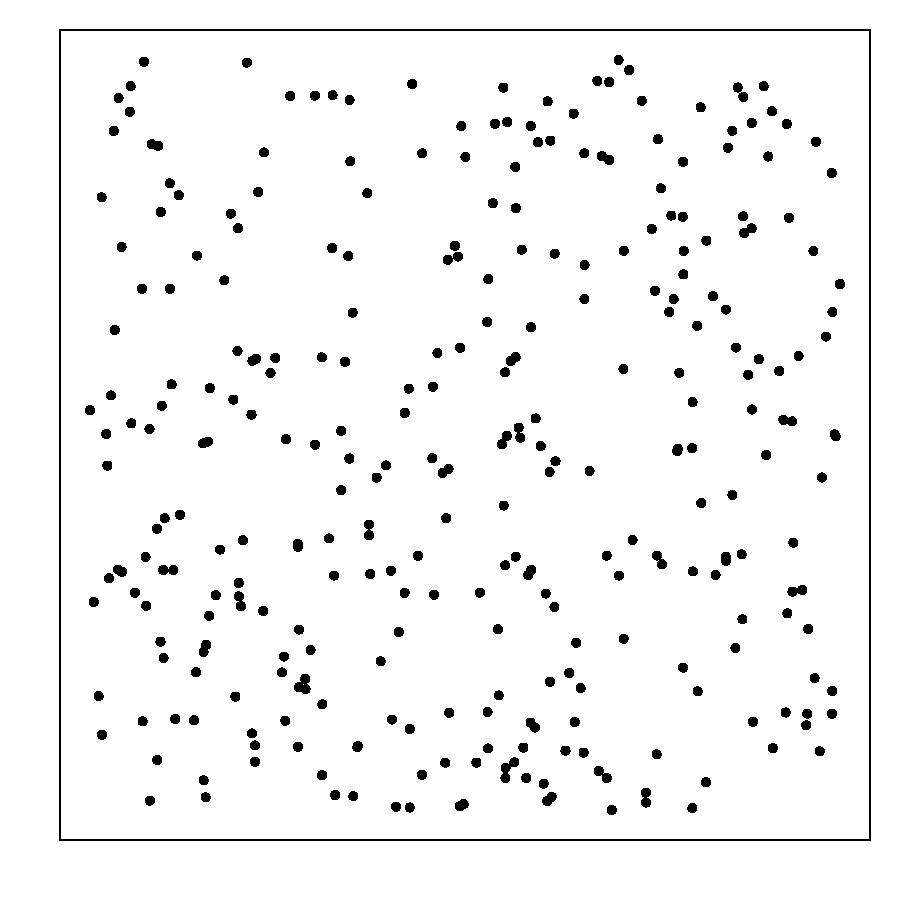
\includegraphics[height=3cm]{Population_study_design/Scatterplots2.pdf}
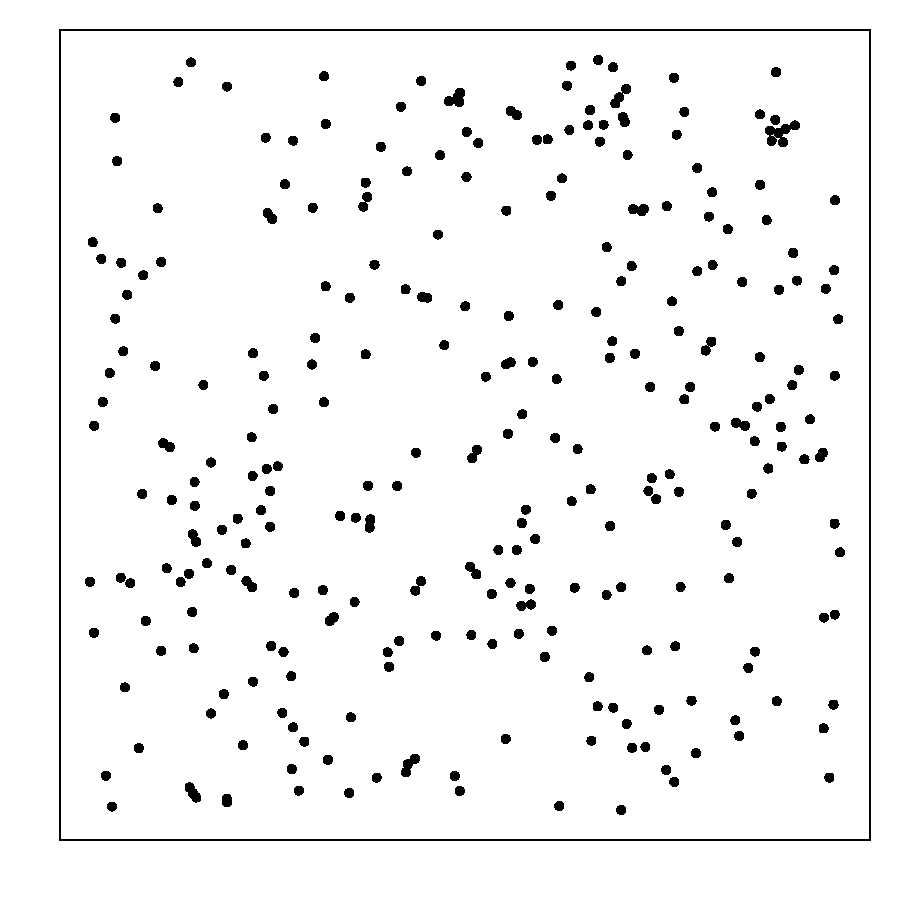
\includegraphics[height=3cm]{Population_study_design/Scatterplots3.pdf}
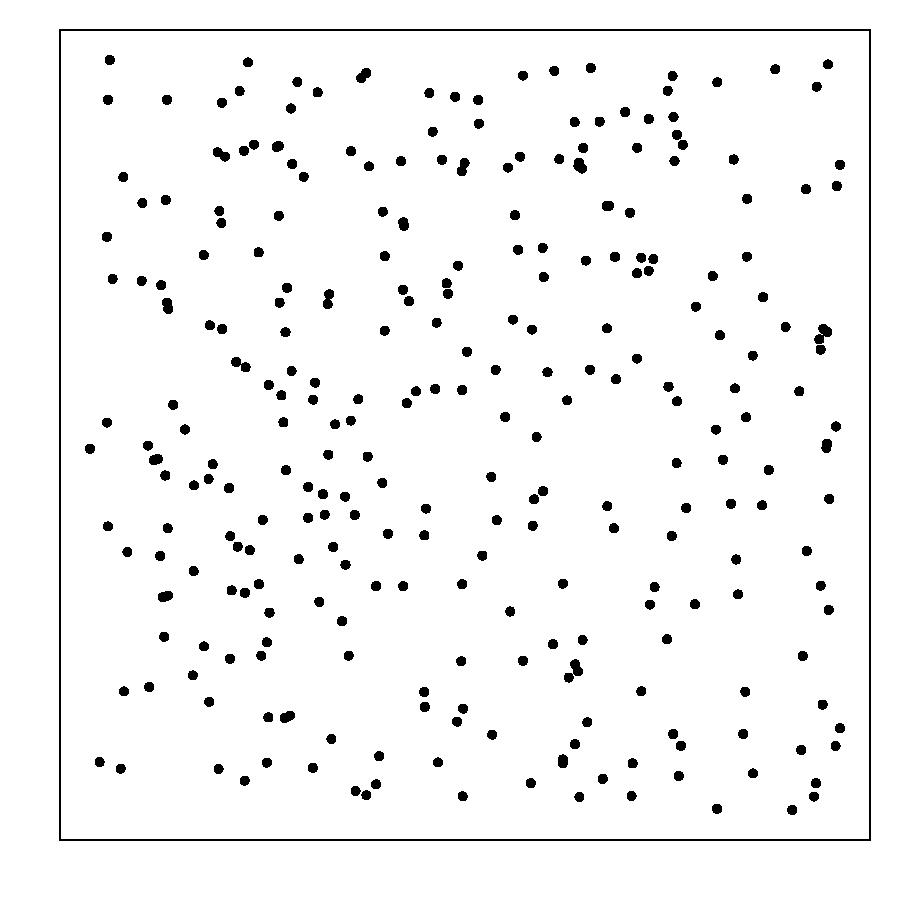
\includegraphics[height=3cm]{Population_study_design/Scatterplots4.pdf}
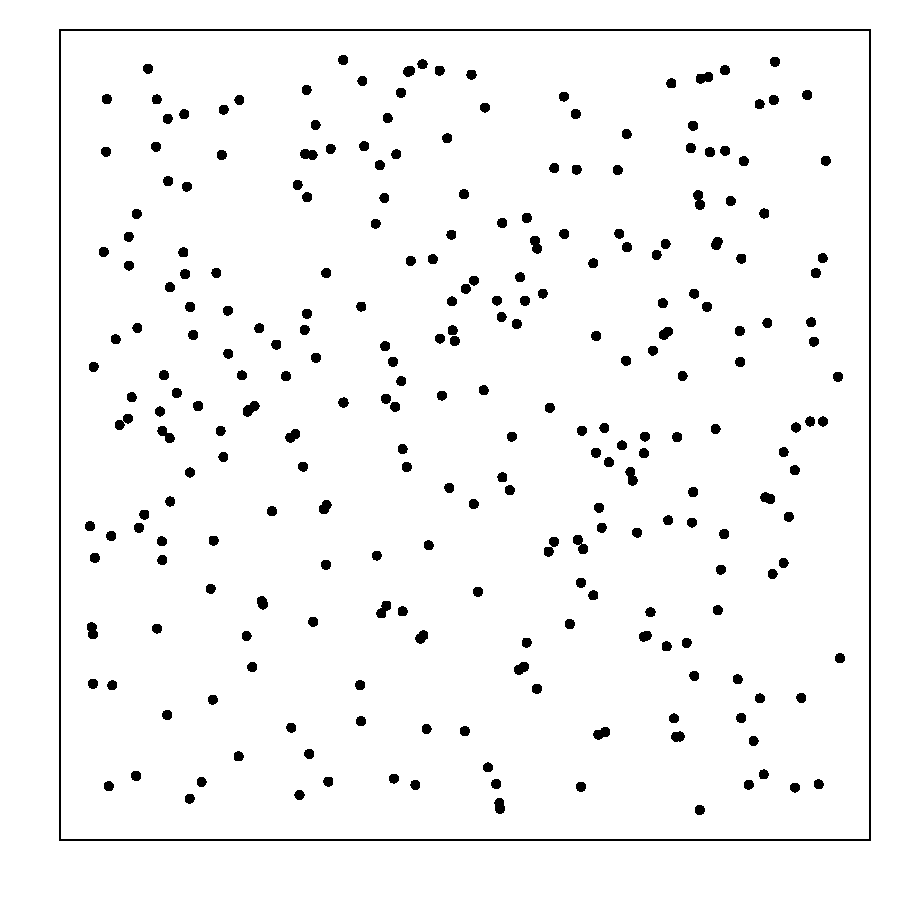
\includegraphics[height=3cm]{Population_study_design/Scatterplots5.pdf}
\end{tcolorbox}


\subsubsection{Triangles}

% Triangles

This domain is another perception example.
The true areas are, respectively, 16, 15, 15, 14 and 14 units.

\begin{tcolorbox}
	Which one of the following triangles do you think has the greatest area?

	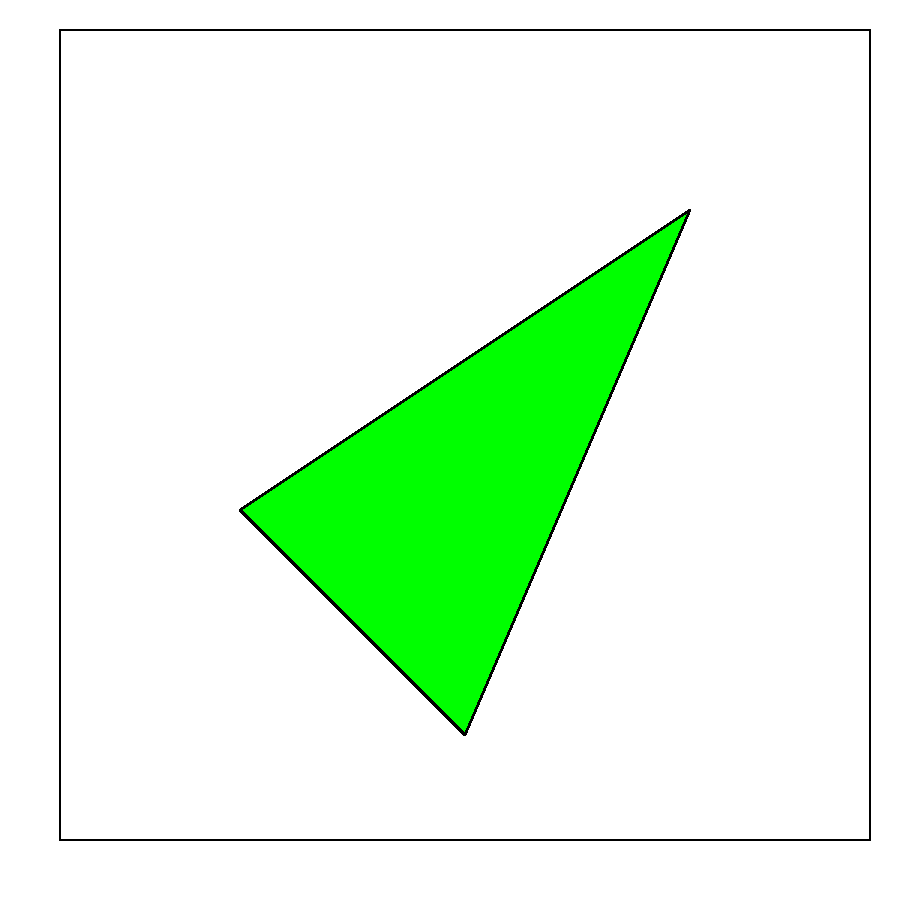
\includegraphics[height=3cm]{Population_study_design/Triangles3.pdf}
	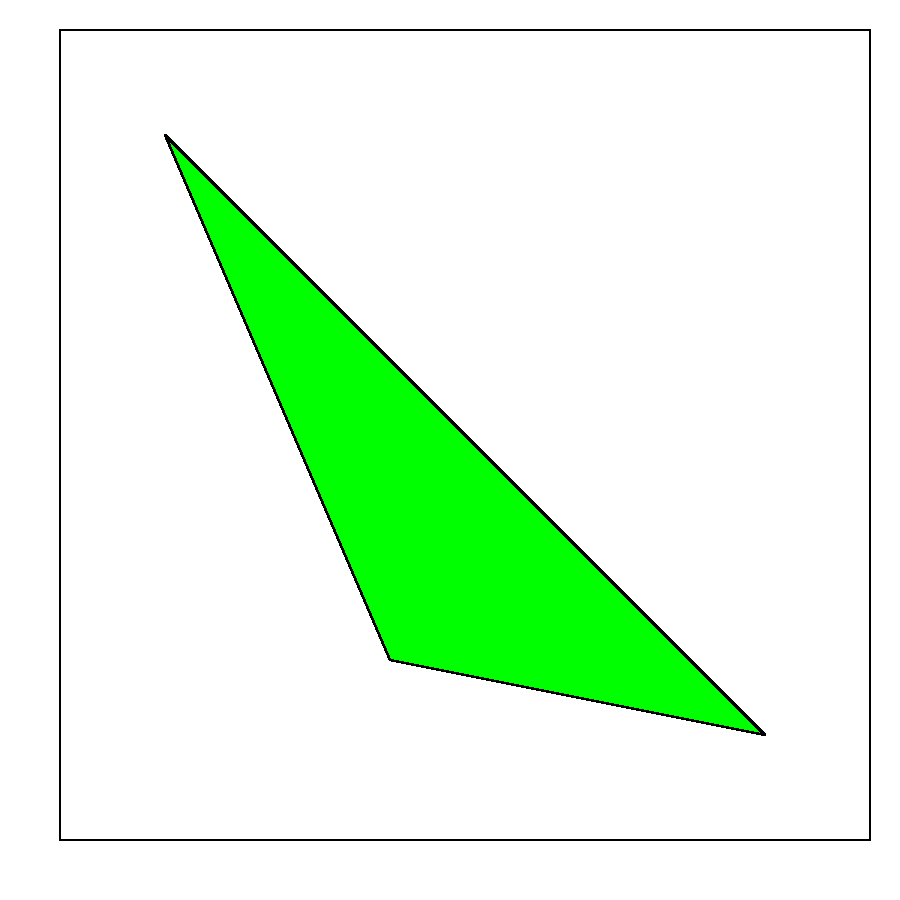
\includegraphics[height=3cm]{Population_study_design/Triangles1.pdf}
	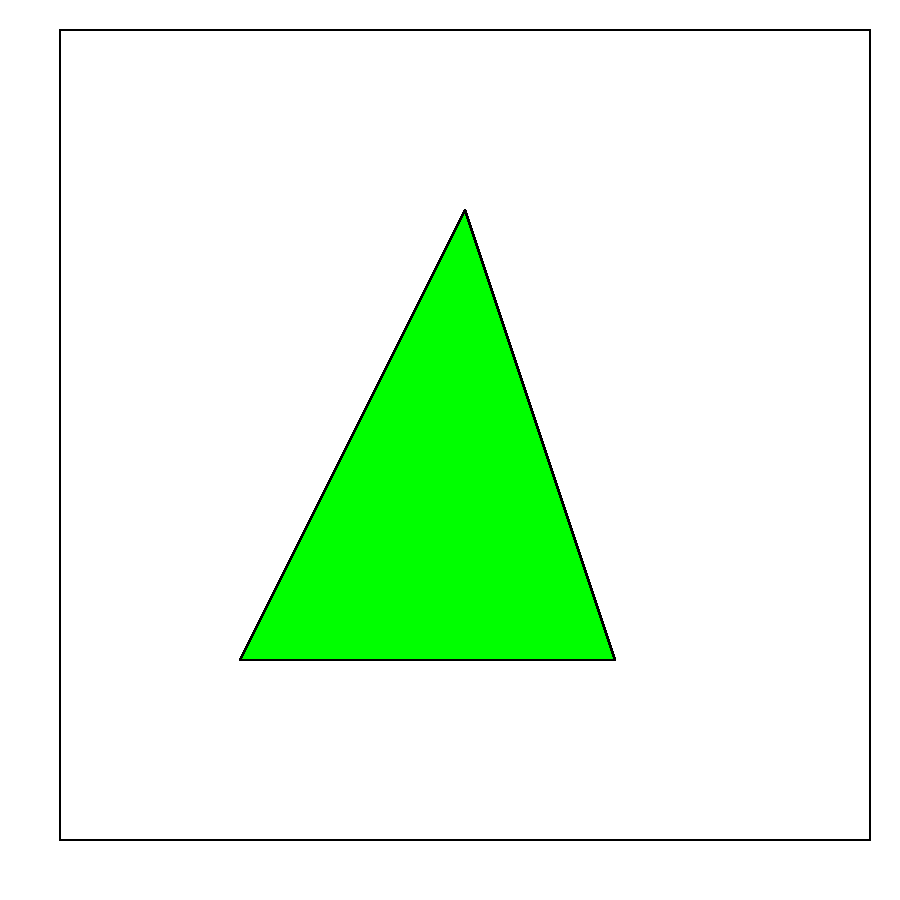
\includegraphics[height=3cm]{Population_study_design/Triangles2.pdf}
	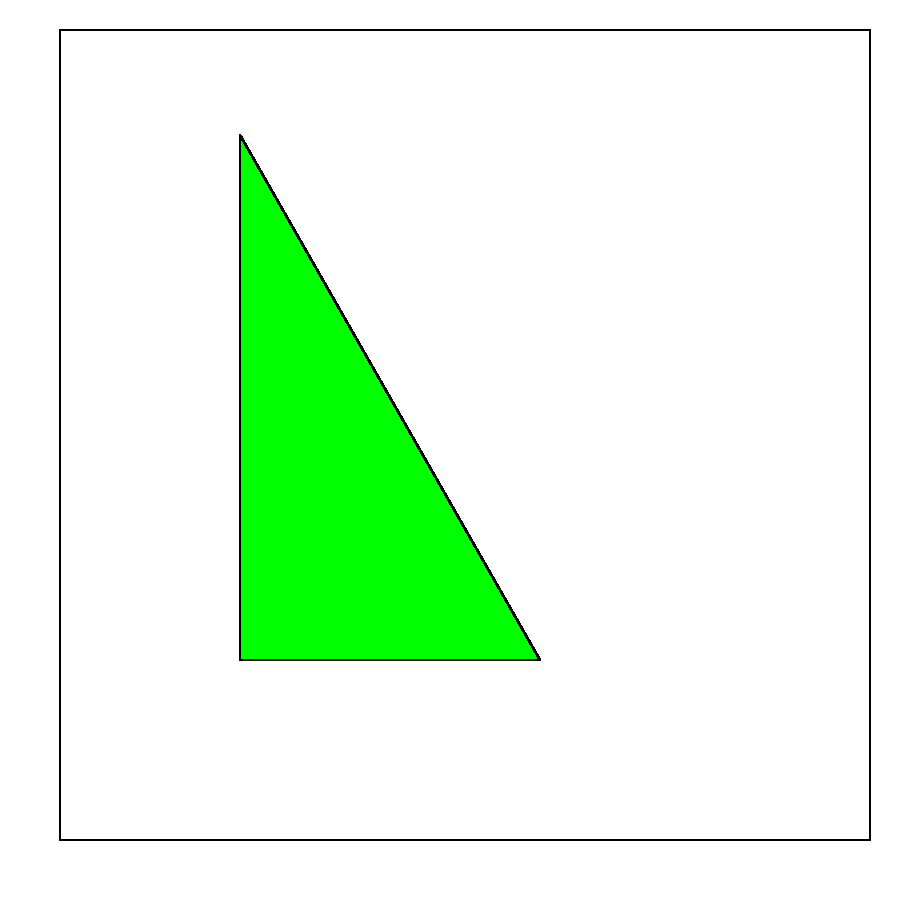
\includegraphics[height=3cm]{Population_study_design/Triangles4.pdf}
	
\includegraphics[height=3cm]{Population_study_design/Triangles5.pdf}	
\end{tcolorbox}


\subsubsection{Population}

% Population

These countries were ranked, respectively, 4th through 8th in terms of population in 2016, when
their populations, in millions, were 258, 206, 202, 186 and 156.

\begin{tcolorbox}
Which one of the following countries do you think has the largest population?

\begin{itemize}
	\setlength\itemsep{-5pt}
	\item Indonesia
	\item Brazil
	\item Pakistan
	\item Nigeria
	\item Bangladesh
\end{itemize}
\end{tcolorbox}


\subsubsection{Surface area}

% Surface area

These countries are ranked, respectively, 2nd through 6th in terms of surface area, including inland bodies of water.
In millions of square kilometres, those surface areas are 9.984, 9.573, 9.525, 8.516 and 7.692.

\begin{tcolorbox}
Which one of the following countries do you think has the greatest surface area, including inland bodies of water?
	
\begin{itemize}
	\setlength\itemsep{-5pt}
	\item Canada
	\item United States of America
	\item China
	\item Brazil
	\item Australia
\end{itemize}
\end{tcolorbox}


\subsection{Objects with two attributes}

Here we describe domains whose choice objects have exactly two real-valued attributes.
In all cases, the levels of these attributes are presented directly to the respondent.
Figure \ref{f:CE} plots the five objects of each of these domains in attribute space, revealing potential conditions for context effects.

\begin{figure}
	\caption{Designs for context effects. Each panel plots the five objects of a domain in attribute space. The domains are, in row major order, Beer, Cars, Restaurants, Flights I, Delayed Choice, Phone Plans, Hotels}\label{f:CE}
	\centering
	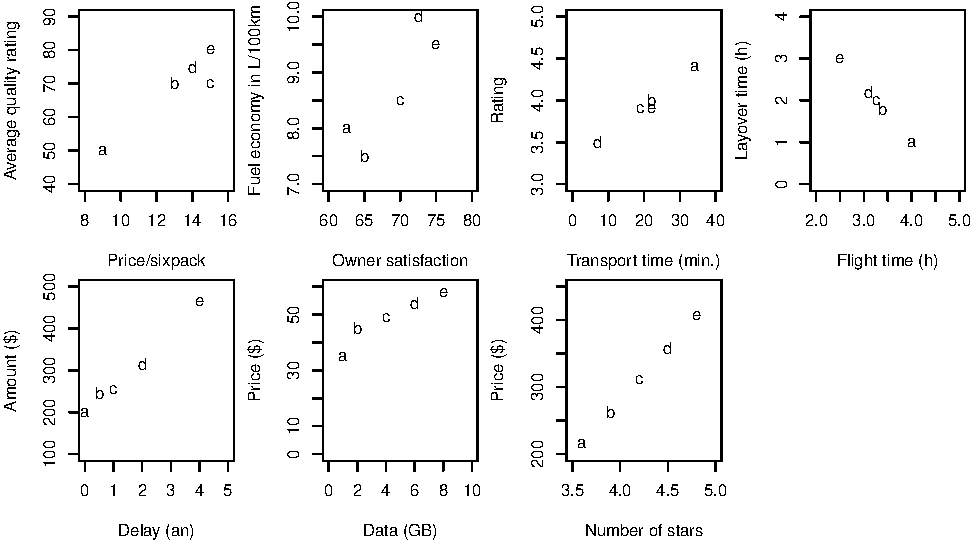
\includegraphics[width=15cm]{./Figures/design_patterns.pdf}
\end{figure}

Table \ref{t:CE} shows, for the first four of these domains, dominance, similarity and betweenness relations that we might expect to generate context effects.
Following usual practice, we exclude similarity relations for two objects in which there is also a dominance relation between the two; and betweenness relations among three objects when two of them are similar and the third is not similar to either of the first two.

\begin{table}
	\centering
	\begin{tabular}{cccc}
		Domain & Dominance & Similarity w/o dominance & Betweenness w/o similarity \\
		\hline
		Beer
		& $e>c$, $b>c$, $d>c$ & $b \sim d$, $d \sim e$, $b \sim e$
		& $a|b|e$ \\
		Cars
		& $a>d$, $b>e$ & & $a|c|b$, $a|c|e$, $a|c|b$, $d|c|e$ \\
		Restaurants
		& $b>e$, $c>e$ & $b \sim c$ & $a|b|d$, $a|c|d$, $a|e|d$ \\
		Flights I 
		& & $b \sim c$, $c \sim d$, $b \sim d$ & $a|b|e$, $a|c|e$, $a|d|e$ \\
		\hline
	\end{tabular}\caption{Relations of dominance, similarity and betweenness in two-attribute domains}\label{t:CE}
\end{table}

\subsubsection{Beer}

% Beer

This domain is from an experiment reported in \citeasnoun{HubePaynPuto82} used to illustrate an asymmetric dominance effect.
The prices are multiplied by 5 and we added choice objects d and e to allow for two more asymmetric dominance effects and two similarity effects.
The first panel of Figure \ref{f:CE} show the choice objects in attribute space.
Table \ref{t:CE} shows the relations of dominance, similarity and betweenness among objects associated with context effects.
The most commonly used domains to illustrate the attraction effect involve Beer, Cars, Apartments, Computers, Restaurants and Televisions.

\begin{tcolorbox}
Below you will find three brands of beer.
You know only the price per sixpack and the average quality ratings made by respondents in a blind taste test.
Given that you had to choose one brand to buy on this information alone, which one would you choose?

\begin{tabular}{cc}
\hline
Price/sixpack & Average quality rating (100 = Best; 0 = Worst) \\ 
\hline
\$9.00 & 50 \\ 
\$13.00 & 70 \\ 
\$15.00 & 70 \\ 
\$14.00 & 75 \\ 
\$15.00 & 80 \\ \hline
\end{tabular}
\end{tcolorbox}


\subsubsection{Cars}

% Cars

This domain is based on an experiment from \citeasnoun{WedePett96}.
There are two experiments involving cars in that article, the experiment in question is  numbered 18 in the appendix to that paper.
Objects below have the same attributes as in that experiment and a similar range of levels.
We adapted the objects to allow for compromise effects.
The second panel of Figure \ref{f:CE} shows the choice objects in attribute space.
Table \ref{f:CE} shows the relations of dominance, similarity and betweenness among objects associated with context effects.

\begin{tcolorbox}
Which one of the following cars would you choose to drive, all other features
begin equal? Ride quality is a on a scale of 0 to 100.

\begin{tabular}{cc}
\hline
Ride quality & Miles per gallon \\ \hline
60 & 30 \\ 
80 & 24 \\ 
70 & 27 \\ 
55 & 28 \\ 
75 & 22 \\ \hline
\end{tabular}
\end{tcolorbox}


\subsubsection{Restaurants}

% Restaurants

This domain is based on another experiment in \citeasnoun{WedePett96}, numbered 19 in the appendix to that paper.
The third panel of Figure \ref{f:CE} shows the choice objects in attribute space.
Table \ref{t:CE} shows the relations of dominance, similarity and betweenness among objects associated with context effects.

\begin{tcolorbox}
Which one of the following restaurants would you choose for your next restaurant meal, based on transportation time (in minutes) and average customer ratings (from
1 to 5).
	
\begin{tabular}{cc}
\hline
Transportation time & Rating \\ \hline
34 & 4.4 \\ 
22 & 4.0 \\ 
19 & 3.9 \\ 
7 & 3.5 \\ 
22 & 3.9 \\ \hline
\end{tabular}
\end{tcolorbox}


\subsubsection{Layovers}

% Layovers

The fourth panel of Figure \ref{f:CE} shows the choice objects in attribute space.
Table \ref{t:CE} shows the relations of dominance, similarity and betweenness among objects associated with context effects.

\begin{tcolorbox}
Which one of the following flight itineraries would you choose?
All involve two flights, with one layover between them.

\begin{tabular}{ccc}
\hline
Total inflight time & Layover time & Total itinerary time \\ \hline
4:00 & 1:00 & 5:00 \\ 
3:24 & 1:48 & 5:12 \\ 
3:15 & 2:00 & 5:15 \\ 
3:06 & 2:12 & 5:18 \\ 
2:30 & 3:00 & 5:30 \\ \hline
\end{tabular}
\end{tcolorbox}


\subsubsection{Delayed Choice}

% Delayed choice

This domain is loosely based on an experiment by \citeasnoun{BenzRapoYagi89}, in which respondents are asked to assign present values equivalent to the receipt of \$200 at time horizons of 0.5, 1, 2 and 4 years.
Based on implied discount factors at various terms, we constructed five choice objects designed to have approximately the same present value equivalent.

\begin{tcolorbox}
Which one of the following would you choose?

\begin{itemize}
	\setlength\itemsep{-5pt}
	\item \$200 credited to your bank account immediately.
	\item \$245 credited to your bank account in six months.
	\item \$255 credited to your bank account in one year.
	\item \$315 credited to your bank account in two years.
	\item \$465 credited to your bank account in four years.
\end{itemize}
\end{tcolorbox}


\subsubsection{Phone plans}

% Phone plans

The source for this domain is the website of Fido Mobile, with rates quoted on March 1, 2017 in Canadian dollars.

\begin{tcolorbox}
Of the following cell phone plans, which one would you choose? In all cases, unlimited calling, text picture and video messages to Canadian and international mobile numbers are included. Excess data usage is billed at \$10 per 500 MB.

\begin{itemize}
	\setlength\itemsep{-5pt}
	\item 1 GB data per month, \$35 per month.
	\item 2 GB data per month, \$45 per month.
	\item 4 GB data per month, \$49 per month.
	\item 6 GB data per month, \$54 per month.
	\item 8 GB data per month, \$58 per month.
\end{itemize}
\end{tcolorbox}


\subsubsection{Hotel rooms}

% Hotel rooms

Using Expedia results, I did a linear regression of price per night on a constant and the Expedia rating, in numbers of stars, for a sample of available hotels.
The five levels of numbers of stars correspond roughly to the mean, plus and minus one sample standard deviation and plus and minus two standard deviations.
Prices are approximately equal to fitted values in the linear regression.

\begin{tcolorbox}
Suppose you are staying over two nights in New York city.
Which one of the following hotels would you choose, based on customer ratings and price per night?	

\begin{itemize}
	\setlength\itemsep{-5pt}
	\item 3.6/5 stars, \$215 per night
	\item 3.9/5 stars, \$263 per night
	\item 4.2/5 stars, \$311 per night
	\item 4.5/5 stars, \$358 per night
	\item 4.8/5 stars, \$406 per night
\end{itemize}
\end{tcolorbox}


\subsection{Objects with multiple attributes}

\subsubsection{Flight itineraries}

% Flight itineraries

This domain illustrates three-way tradeoffs.
The points form a constellation in the simplex that resembles the pattern of points on the ``five'' side of a die.

\begin{tcolorbox}
Which one of the following flight itineraries would you choose? All involve two
flights and have a total duration of six hours.

\begin{tabular}{ccc}
\hline
	1st flight & Layover & 2nd flight \\ \hline
	1:30 & 1:15 & 3:15 \\ 
	3:15 & 1:15 & 1:30 \\ 
	2:15 & 1:30 & 2:15 \\ 
	1:30 & 1:45 & 2:45 \\ 
	2:45 & 1:45 & 1:30 \\ \hline
\end{tabular}
\end{tcolorbox}


\subsubsection{Televisions}

% Televisions

The source for this domain is the website of Best Buy Canada, with prices in Canadian dollars.

\begin{tcolorbox}
Which one of the following televisions would you choose to buy if you
were in the market for a television? All are LED televisions. Resolution
refers to number of horizontal lines. Smart indicates internet connectivity.

\begin{tabular}{ccccccc}
\hline
Brand & Resolution & Smart & Price (\$) & Screen Size (inches) &  \\ \hline
Sharp & 1080 & Yes & 309 & 32 &  \\ 
Insignia & 720 & No & 209 & 32 &  \\ 
Sony & 720 & Yes & 439 & 32 &  \\ 
Samsung & 1080 & Yes & 459 & 40 &  \\ 
Toshiba & 1080 & No & 409 & 43 &  \\
\hline
\end{tabular}
\end{tcolorbox}


\subsubsection{Coffee}

% Coffee

The source for this domain is the website \texttt{buycoffeecanada.com}, with prices in Canadian dollars.

\begin{tcolorbox}
You need to buy 16oz of ground coffee for a brunch with friends.
Which one of the following ground coffees would you choose?

\begin{tabular}{rcl}
\hline
Price & Fair Trade & Name: Description \\
\hline
18.71 & Yes & Ethiopian Yirgacheffe: vibrant and intensely aromatic, fruity \\
9.99 & No & Colombian Supremo: mellow cup, complex aromas and rich flavours \\
13.72 & Yes & Colombian Organic: medium body, fragrant aroma and mild acidity \\
12.35 & No & Tanzania Peaberry: full bodied coffee, chocolatey aroma, wine-like finish \\
13.46 & No & Sumatra Mandheling: exotic, earthy, bright with low acidity \\
\hline
\end{tabular}
\end{tcolorbox}


\subsubsection{Charity}

% Charity

The charities in this domain are real charities.
The first two are relatively innocuous in the sense that most people support the goals of both.
However, the Canadian Cancer Society attracts much more financial support than Arthritis Research Canada and we might expect that most people would prefer a marginal dollar going to the former.
The two other charities have goals that are nearly opposite and elicit strong emotions (of different kinds) from some.

\begin{tcolorbox}
Suppose someone was donating a total of 100 dollars to a combination of charities,
on your behalf.
Which one of the following divisions of the 100 dollars would you choose?

\begin{tabular}{p{35mm}|p{35mm}|p{35mm}|p{35mm}}
\hline
Arthritis Research Canada &
Canadian Cancer Society &
Canadian Coalition for Firearm Rights &
Coalition for Gun Control \\
\hline
90 & 10 & 0 & 0 \\
35 & 60 & 5 & 0 \\
35 & 60 & 0 & 5 \\
10 & 80 & 10 & 0 \\
10 & 80 & 0 & 10 \\
\hline
\end{tabular}
\end{tcolorbox}


\section{Comments of respondents}

\bibliographystyle{oupecon}
\bibliography{bibliography}

\end{document}